\documentclass{beamer}  
\usepackage{../slides}
\usepackage{cancel}
\usepackage{appendixnumberbeamer}
\setbeameroption{hide notes}
\defbeamertemplate{description item}{align left}{\insertdescriptionitem\hfill}

%%%%%%%%%%%%%%%%%%%% Not needed at home!
\usepackage[compatibility=false]{caption}
\usepackage{subcaption}
%%%%%%%%%%%%%%%%%%%% Not needed at home!


\title[Binary Regressors]{Estimating the Effect of a Mis-measured, Endogenous, Binary Treatment}
\author[FJ DiTraglia]{Francis J.\ DiTraglia\\ Camilo Garcia-Jimeno}
\institute{University of Pennsylvania}
\date{December 6th, 2016}
\begin{document} 
%%%%%%%%%%%%%%%%%%%%%%%%%%%%%%%%%%%%%%%%

\begin{frame}[plain]
	\titlepage 
\end{frame} 
%%%%%%%%%%%%%%%%%%%%%%%%%%%%%%%%%%%%%%%%%
\begin{frame}
  \frametitle{What is the causal effect of $T^*$?}
  \vspace{-1em}
  \[ y_i = h(T^*_i, \mathbf{x}_i) + \varepsilon_i\]
  \vspace{-1.5em}
  \begin{itemize}
    \item $y$ -- Outcome of interest
    \item $h$ -- Unknown function that \emph{does not depend on} $i$
    \item $T^*$ -- Unobserved, endogenous binary treatment
    \item $T$ -- Observed, mis-measured binary surrogate for $T^*$
    \item $\mathbf{x}$ -- Exogenous covariates
    \item $\varepsilon$ -- Mean-zero error term
    \item $z$ -- Discrete (typically binary) instrumental variable
  \end{itemize}

 \begin{block}{Target of Inference:}
   ATE function:  $\alert{\tau(\mathbf{x}) = h(1,\mathbf{x}) - h(0,\mathbf{x})}$
  \end{block}
\end{frame}
%%%%%%%%%%%%%%%%%%%%%%%%%%%%%%%%%%%%%%%%%
\begin{frame}
  \frametitle{Example: Smoking and Birthweight (SNAP Trial)}
\framesubtitle{Coleman et al.\ (N Engl J Med, 2012)}
  RCT with 1050 pregnant smokers in England: 521 given nicotine patches, the rest given placebo patches.
\begin{itemize}
  \item $y$ -- Birthweight 
  \item $T^*$ -- True smoking behavior 
  \item $T$ -- Self-reported smoking behavior
  \item $\mathbf{x}$ -- Mother characteristics
  \item $z$ -- Indicator of nicotine patch
\end{itemize}
   
\end{frame}
%%%%%%%%%%%%%%%%%%%%%%%%%%%%%%%%%%%%%%%%%%
\begin{frame}
  \frametitle{Example: Schooling and Test Scores}
\framesubtitle{Burde \& Linden (2013, AEJ Applied)}
  RCT in Afghanistan: 32 villages divided into 11 clusters. Randomly choose 6 and set up school in each village of these clusters.

\begin{itemize}
  \item $y$ -- Child's score on math and language test 
  \item $T^*$ -- Child's true school attendance
  \item $T$ -- Parent's report of child's school attendance
  \item $\mathbf{x}$ -- Child and household characteristics
  \item $z$ -- School built in village
\end{itemize}
\end{frame}
%%%%%%%%%%%%%%%%%%%%%%%%%%%%%%%%%%%%%%%%%%%%
%\begin{frame}
%  \frametitle{Example: Job Training Partnership Act (JPTA)}
%\framesubtitle{Heckman et al.\ (2000, QJE)}
%Randomized offer of job training, but about $30\%$ of those \emph{not} offered also obtain training and about $40\%$ of those offered training don't attend. Estimate causal effect of \emph{training} rather than \emph{offer} of training.
%
%\begin{itemize}
%  \item $y$ -- Log wage 
%  \item $T^*$ -- True training attendence
%  \item $T$ -- Self-reported training attendance
%  \item $\mathbf{x}$ -- Individual characteristics
%  \item $z$ -- Offer of job training
%\end{itemize}
%   
%\end{frame}
%%%%%%%%%%%%%%%%%%%%%%%%%%%%%%%%%%%%%%%%%%%
\begin{frame}
  \frametitle{Example: Returns to Schooling} 
\framesubtitle{Oreopoulos (2006, AER)}
Fuzzy RD: minimum school-leaving age in UK increased from 14 to 15 in 1947 but some already stayed until 15 before the law and others failed to comply after it.
\begin{itemize}
  \item $y$ -- Log wage 
  \item $T^*$ -- School attendance at age 15
  \item $T$ -- Self-report of school attendance at age 15
  \item $\mathbf{x}$ -- Individual characteristics
  \item $z$ -- Indicator: born in or after 1933
\end{itemize}
   
\end{frame}
%%%%%%%%%%%%%%%%%%%%%%%%%%%%%%%%%%%%%%%%%%%
\begin{frame}[label=MAHAJAN_BODY]
  \frametitle{Related Literature}
 
  \begin{block}{Continuous Treatment}
    \small
  Lewbel (1997, 2012), Schennach (2004, 2007), Chen et al. (2005), Hu \& Schennach (2008), Song (2015), Hu et al.\ (2015)\ldots 
  \end{block}

  \begin{block}{Binary, Exogenous Treatment}
    \small
   Aigner (1973), Bollinger (1996), Kane et al. (1999), Black et al. (2000), Frazis \& Loewenstein (2003), Mahajan (2006), Lewbel (2007) 
  \end{block}

  \begin{block}{Binary, Endogenous Treatment}
    \alert{Mahajan (2006)}, \small Shiu (2015), Ura (2015) 
  \end{block}
    \hyperlink{MAHAJAN_APPEND}{\beamergotobutton{Mahajan Details}}
\end{frame}
%%%%%%%%%%%%%%%%%%%%%%%%%%%%%%%%%%%%%%%
%\begin{frame}
%  \frametitle{Model: $y = h(T^*, \mathbf{x}) + \varepsilon$}
%  \begin{block}{ATE Function}
%   $ \tau(\mathbf{x}) = h(1,\mathbf{x}) - h(0, \mathbf{x})$
%  \end{block}
%  \begin{block}{First-stage}
%    $p^*_k(\mathbf{x}) \equiv \mathbb{P}(T^*=1|z=z_k,\mathbf{x}) \neq \mathbb{P}(T^*=1|z=z_\ell, \mathbf{x})\equiv p_\ell^*(\mathbf{x}) $, $k\neq \ell$
%  \end{block}
%  \begin{block}{Measurement Error}
%    Non-differential, $\mathbb{E}[\varepsilon|T^*,T,z,\mathbf{x}] =  \mathbb{E}[\varepsilon|T^*,z,\mathbf{x}]$, and does not depend on $z$:
%\begin{eqnarray*}
% \alpha_0(\mathbf{x})&=&  \mathbb{P}(T = 1| T^* = 0, z, \mathbf{x})  \\ 
% \alpha_1(\mathbf{x})&=& 
%  \mathbb{P}(T = 0| T^* = 1, z, \mathbf{x}) 
%\end{eqnarray*}
%    
%  \end{block}
%\end{frame}
%%%%%%%%%%%%%%%%%%%%%%%%%%%%%%%%%%%%%%%
%\begin{frame}
%  \frametitle{Notation}
%
%  \begin{itemize}
%    \item Treat exog.\ covariates $\mathbf{x}$ non-parametrically: hold fixed at $\mathbf{x}_a$ throughout:
%      \vspace{-1em}
%      \begin{eqnarray*}
%        y &=&  \beta T^* + u\\
%        u &=&  \varepsilon + c
%      \end{eqnarray*}
%      where $\beta = \tau(\mathbf{x}_a)$ and $c = h(0,\mathbf{x}_a)$.
%    \item Similarly:
%      \begin{eqnarray*}
%        \alpha_0 &=&  \mathbb{P}(T=1|T^*=0)\\
%        \alpha_1 &=&  \mathbb{P}(T=0|T^*=1)\\
%        p_k^* &=&  \mathbb{P}(T^* = 1|z=z_k)
%      \end{eqnarray*}
%  \end{itemize}
%\end{frame}
%%%%%%%%%%%%%%%%%%%%%%%%%%%%%%%%%%%%%%%
\begin{frame}
  \frametitle{Model: $y = c + \beta T^* + \varepsilon$}

  \begin{block}{Valid Instrument}
    $\mathbb{E}[\varepsilon|z] =0$. 
  \end{block}

  \begin{block}{First-stage}
    $p^*_k \equiv \mathbb{P}(T^*=1|z=z_k) \neq \mathbb{P}(T^*=1|z=z_\ell)\equiv p_\ell^*$, $k\neq \ell$
  \end{block}

  \begin{block}{Non-differential Measurement Error}
    \begin{itemize}
      \item $\mathbb{E}[\varepsilon|T^*,T,z] =  \mathbb{E}[\varepsilon|T^*,z]$
      \item $\alpha_0 = \mathbb{P}(T = 1| T^* = 0, z)$ 
      \item  $\alpha_1 = \mathbb{P}(T = 0| T^* = 1, z)$ 
      \item $\alpha_0 + \alpha_1 < 1$ 
    \end{itemize}
  \end{block}


\end{frame}
%%%%%%%%%%%%%%%%%%%%%%%%%%%%%%%%%%%%%%
\begin{frame}
  \frametitle{Observable Moments:  $y = c + \beta T^* + \varepsilon$}

\phantom{Define error term that absorbs constant: $u = c + \varepsilon$}

\begin{center}
  \begin{tabular}{c|c|c|c|c|}
    \multicolumn{1}{c}{}& \multicolumn{1}{c}{$z=1$} &\multicolumn{1}{c}{$z=2$} & \multicolumn{1}{c}{\dots} &\multicolumn{1}{c}{$z=K$}\\
    \cline{2-5}
    $T=0$ & \diagbox[dir=NE]{$\bar{y}_{01}$}{$p_{01}$} & \diagbox[dir=NE]{$\bar{y}_{02}$}{$p_{02}$} & \dots &\diagbox[dir=NE]{$\bar{y}_{0K}$}{$p_{0K}$}\\
    \cline{2-5}
    $T=1$ & \diagbox[dir=NE]{$\bar{y}_{11}$}{$p_{11}$} & \diagbox[dir=NE]{$\bar{y}_{12}$}{$p_{12}$} & \dots &\diagbox[dir=NE]{$\bar{y}_{1K}$}{$p_{1K}$}\\
    \cline{2-5}
  \end{tabular}
\end{center}

\vspace{1em}

\[\bar{y}_{tk} = \mathbb{E}[y|T=t,z=z_k],
\quad p_{tk} =q_k p_k\]
\small
\[q_k = \mathbb{P}(z = z_k), \quad
p_k = \mathbb{P}(T=1|z=z_k)\]

\end{frame}

%%%%%%%%%%%%%%%%%%%%%%%%%%%%%%%%%%%%%%
\begin{frame}
  \frametitle{Unobservable Moments: $y = \beta T^* + u$}

\alert{Define error term that absorbs constant: $u = c + \varepsilon$}

\begin{center}
  \begin{tabular}{c|c|c|c|c|}
    \multicolumn{1}{c}{}& \multicolumn{1}{c}{$z=1$} &\multicolumn{1}{c}{$z=2$} & \multicolumn{1}{c}{\dots} &\multicolumn{1}{c}{$z=K$}\\
    \cline{2-5}
    $T^*=0$ & \diagbox[dir=NE]{$m^*_{01}$}{$p^*_{01}$} & \diagbox[dir=NE]{$m^*_{02}$}{$p^*_{02}$} & \dots &\diagbox[dir=NE]{$m^*_{0K}$}{$p^*_{0K}$}\\
    \cline{2-5}
    $T^*=1$ & \diagbox[dir=NE]{$m^*_{11}$}{$p^*_{11}$} & \diagbox[dir=NE]{$m^*_{12}$}{$p^*_{12}$} & \dots &\diagbox[dir=NE]{$m^*_{1K}$}{$p^*_{1K}$}\\
    \cline{2-5}
  \end{tabular}
\end{center}

\vspace{1em}

\[m^*_{tk} = \mathbb{E}[u|T^*=t,z=z_k],
\quad p^*_{tk}=q_k p^*_k\]
\small
\[q_k = \mathbb{P}(z = z_k),\quad p^*_k=\mathbb{P}(T^*=1|z=z_k)\]

\end{frame}
%%%%%%%%%%%%%%%%%%%%%%%%%%%%%%%%%%%%%%
%\begin{frame}
%  \frametitle{Unrestricted System of Equations} 
%  \begin{eqnarray*}
%   (1 - p_k) \bar{y}_{0k} &\equiv& \alert{\widetilde{y}_{0k}= (\beta + m_{1k}^*) \alpha_1 p_k^*  + (1 -\alpha_0)(1 - p^*_k)m_{0k}^* } \\
%    p_k \bar{y}_{1k} &\equiv&  \alert{\widetilde{y}_{1k}=(\beta + m_{1k}^*) (1 - \alpha_1)p_k^* + \alpha_0 (1 - p_k^*) m_{0k}^*} 
%  \end{eqnarray*}
%  \small
%  \[p^*_k =  \frac{p_k - \alpha_0}{1 - \alpha_0 - \alpha_1} \]
%
%\end{frame}
%%%%%%%%%%%%%%%%%%%%%%%%%%%%%%%%%%%%%%
\begin{frame}
  \frametitle{Possible Restrictions On $m^*_{tk}$}
  \begin{block}{Joint Exogeneity: $\mathbb{E}[\varepsilon|T^*,z]=0$}
    $\implies m^*_{tk} =c \quad$ for all $t,k$
  \end{block}
  \begin{block}{Exogenous Treatment: $\mathbb{E}[\varepsilon|T^*]=0$}
    $\implies \displaystyle \frac{1}{\mathbb{P}(T^*=t)}\sum_{k}p^*_{tk}m^*_{tk} = c\quad$  for all $t$
  \end{block}
  \begin{alertblock}{Exogenous Instrument: $\mathbb{E}[\varepsilon|z]=0$}
    $\implies (1-p^*_k)m^*_{0k} + p^*_k m^*_{1k}=c \quad$ for all $k$
  \end{alertblock}

\end{frame}
%%%%%%%%%%%%%%%%%%%%%%%%%%%%%%%%%%%%%%
\begin{frame}
  \frametitle{System of Equations given $E[\varepsilon|z]=0$}
  \alert{\framebox{$\mathbb{E}[\varepsilon|z]=0 \implies$ \emph{pair} of equations for each $k = 1, \dots, K$}}
\begin{align*}
  \hat{y}_{0k} &=\alpha_1(p_k - \alpha_0)\left(\frac{\beta}{1 - \alpha_0 - \alpha_1}\right) + (1-\alpha_0)c - (p _k -  \alpha_0)m_{1k}^* \\[1.5ex]
  \label{eq:MC1IV}
  \hat{y}_{1k} &=(1-\alpha_1)(p_k - \alpha_0)\left(\frac{\beta}{1 - \alpha_0 - \alpha_1}\right) + \alpha_0 c + (p _k -  \alpha_0)m_{1k}^*
\end{align*}

\vspace{0.5em}
where $\hat{y}_{0k}=(1-p_k)\bar{y}_{0k}$ and $\hat{y}_{0k}=p_k\bar{y}_{1k}$


\vspace{2em} 

\hfill \alert{\framebox{$2K$ Equations in $K+4$ Unknowns}}
\end{frame}
%%%%%%%%%%%%%%%%%%%%%%%%%%%%%%%%%%%%%
\begin{frame}
  \frametitle{$\beta$ is undentified regardless of $K$.}
  \framesubtitle{Proof of special case: $\alpha_0 = 0$}
    \begin{enumerate}
      \item System of equations: 
        \vspace{-0.5em}
\begin{align*}
  \widetilde{y}_{0k} &=c + p_k \alert{ \left(\frac{\beta\alpha_1}{1 -  \alpha_1}\right)} - p _k m_{1k}^* \\
  \widetilde{y}_{1k} &=p_k \beta + p _k m_{1k}^*
\end{align*}
  \item $\beta/(1-\alpha_1) \equiv \beta_{IV}$ identified,  $\beta\alpha_1/(1-\alpha_1) = \alert{\beta_{IV} - \beta} \implies$ 
        \vspace{-0.5em}
\begin{align*}
  \textcolor{blue}{(c + p_k \beta_{IV} - \widetilde{y}_{0k})}/p_k &=\beta + m_{1k}^* \\
  \widetilde{y}_{1k}/p_k &= \beta + m_{1k}^*
\end{align*}
\item Sum equations from 1.\ $\implies (c + p_k \beta_{IV} - \widetilde{y}_{0k}) = \textcolor{blue}{\widetilde{y}_{1k}}$
    \end{enumerate}
    
\end{frame}
%%%%%%%%%%%%%%%%%%%%%%%%%%%%%%%%%%%%%%
\begin{frame}
  \frametitle{Bounds for Mis-classification Probabilities}


  \begin{block}{$\alpha_0(z) = \alpha_0, \; \alpha_1(z) =\alpha_1$ }
  \[
    \implies \quad p_k^* = \frac{p_k - \alpha_0}{1 - \alpha_0 - \alpha_1}, \quad
  1 - p_k^* = \frac{1 - p_k - \alpha_1}{1 - \alpha_0 - \alpha_1}\]
  \end{block}

  \begin{block}{$\alpha_0 + \alpha_1 < 1\iff \mbox{Cor}(T,T^*)>0 \iff (1 - \alpha_0 - \alpha_1) > 0$}
  \end{block}

  \begin{alertblock}{$\alpha_0 < \min_k \{p_k\}, \; \alpha_1 < \min_k \{1 - p_k\}$}
  \end{alertblock}
  
\end{frame}
%%%%%%%%%%%%%%%%%%%%%%%%%%%%%%%%%%%%%%
\begin{frame}[plain, c]
  \frametitle{$\alpha_0 \leq \min_k \left\{p_k\right\}, \; \; \alpha_1 \leq \min_k \left\{1 - p_k\right\}$}
\begin{figure}[h]
  \centering
  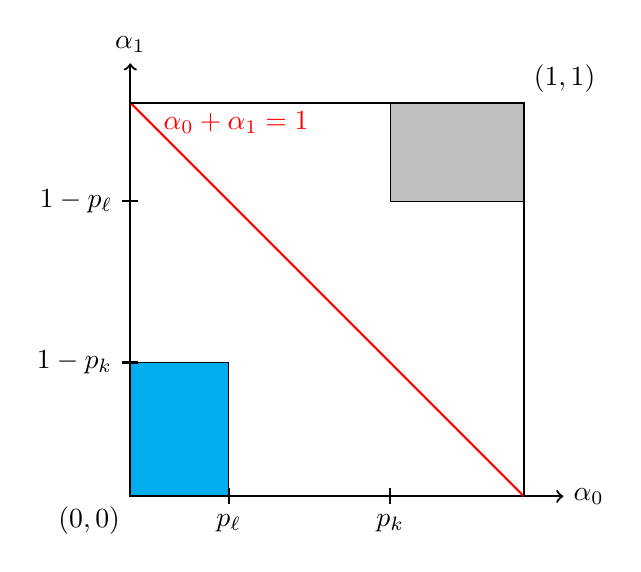
\begin{tikzpicture}[scale=5]
    \draw [fill = lightgray] (0.66,0.75) rectangle (1,1);
    \draw [fill = cyan] (0,0) rectangle (0.25, 0.34);
    \draw [thick, <->] (0,1.1)
    node[above] {$\alpha_1$} -- (0,0) 
    node [below left] {$(0,0)$} -- (1.1,0) 
    node [right] {$\alpha_0$};
    \draw [thick] (0.25,0.02) -- (0.25,-0.02) node [below] {$p_\ell$}; 
    \draw [thick] (0.02,0.75) -- (-0.02,0.75) node [left] {$1 - p_\ell$}; 
    \draw [thick] (0.66,0.02) -- (0.66,-0.02) node [below] {$p_k$}; 
    \draw [thick] (0.02,0.34) -- (-0.02,0.34) node [left] {$1 - p_k$}; 
    \draw [thick, red] (0,1) to (1,0); 
    \node [right, red] at (0.06,0.95) {$\alpha_0 + \alpha_1 = 1$};
    \draw [thick] (0,1) -- (1,1) -- (1,0);
    \node [above right] at (1,1) {$(1,1)$};
    \end{tikzpicture}
\end{figure}
\end{frame}
%%%%%%%%%%%%%%%%%%%%%%%%%%%%%%%%%%%%%%
\begin{frame}
  \frametitle{Bounds for $\beta$}
  \begin{block}{$\mathbb{E}[\varepsilon|z]=0$} 
    $\implies \beta_{RF} = \mathbb{E}[y|z_k] - \mathbb{E}[y|z_\ell] =\beta (p_k^* - p_\ell^*)$
  \end{block}

  \begin{block}{Mis-classification} 
  $\implies p_k^* - p_\ell^* = (p_k - p_\ell)/(1 - \alpha_0 - \alpha_1)$
  \end{block}

  \vspace{1em}

  \begin{alertblock}{Combining: $\beta_{IV} = \beta / (1 - \alpha_0 - \alpha_1)$}
  \end{alertblock}

  \vspace{-1em}

\begin{block}{$\alpha_0 + \alpha_1 < 1 \implies $}
  \begin{itemize}
    \item $\beta$ is between $\beta_{RF}$ and $\beta_{IV}$ 
    \item $\beta_{IV}$ \emph{inflated} but has correct sign 
    \item $\beta_{RF}$ bound equivalent to substituting $\alpha_0, \alpha_1$ bounds
  \end{itemize}
\end{block}
  
\end{frame}
%%%%%%%%%%%%%%%%%%%%%%%%%%%%%%%%%%%%%%
\begin{frame}
  \frametitle{Strengthening the Measurement Error Assumptions}

  \begin{itemize}
    \item $\alpha_0 = \mathbb{P}(T=1|T^*=0, z)$
    \item $\alpha_1 = \mathbb{P}(T=0|T^*=1, z)$
    \item $\alpha_0 + \alpha_1 < 1$
    \item \alert{$\mathbb{E}[\varepsilon|T^*,T,z] = \mathbb{E}[\varepsilon|T^*,z]$}
  \end{itemize}


  \begin{block}{Additional Assumption}
    $\mathbb{E}[\varepsilon^2|T^*,T,z] = \mathbb{E}[\varepsilon^2|T^*,z]$
  \end{block}

  \vspace{1em}
  \hfill\alert{Improve bounds for $\alpha_0, \alpha_1$ to tighten lower bound for $\beta$\ldots}


%   \begin{alertblock}{Stronger}
 %     $\varepsilon$ conditionally independent of $T$ given $T^*$ and $z$.
 % \end{alertblock}

  
\end{frame}
%%%%%%%%%%%%%%%%%%%%%%%%%%%%%%%%%%%%%%
\begin{frame}
  \frametitle{Tighter Bounds for $\alpha_0, \alpha_1$ from Conditional Variances}
  \begin{block}{Assume}
    $\mathbb{E}[\varepsilon^2|T^*,T,z] = \mathbb{E}[\varepsilon^2|T^*,z]$
  \end{block}

  \begin{block}{Observables}
    $\sigma^2_{tk} = \mbox{Var}(y|T=t,z=k)$ 
  \end{block}

  \begin{block}{Constrain Unobservables}
    $s^{*2}_{tk} = Var(u|T^*=t, z_k) > 0$ 

    \footnotesize
\begin{align*}
  (p_k - \alpha_0) \left[ (1 - \alpha_0)p_k \sigma^2_{1k} - \alpha_0 (1 - p_k)\sigma_{0k}^2 \right] &> \alpha_0 (1 - \alpha_0)p_k (1 - p_k)(\bar{y}_{1k} - \bar{y}_{0k})^2\\
  (1 - p_k - \alpha_1) \left[ (1 - \alpha_1)(1 - p_k) \sigma^2_{0k} - \alpha_1 p_k\sigma_{1k}^2 \right] &> \alpha_1 (1 - \alpha_1)p_k (1 - p_k)(\bar{y}_{1k} - \bar{y}_{0k})^2
\end{align*}
  \end{block}
\end{frame}
%%%%%%%%%%%%%%%%%%%%%%%%%%%%%%%%%%%%%%

\begin{frame}[c]
  \frametitle{Schooling and Test Scores -- Afghan RCT}
  \framesubtitle{Burde \& Linden (2013, AEJ Applied)}
\begin{columns}[c]
  \begin{column}{0.4\textwidth}
    \begin{block}{``Weak'' Bounds}
      $\beta \in [0.65 \times\beta_{IV},\; \beta_{IV}]$
    \end{block}
    \vspace{1em}
    \begin{alertblock}{Add 2nd Moments}
      $\beta \in [0.78 \times \beta_{IV},\;\beta_{IV}]$
    \end{alertblock}
  \end{column}
  \begin{column}{0.6\textwidth}
      \begin{figure}[h]
        \centering
        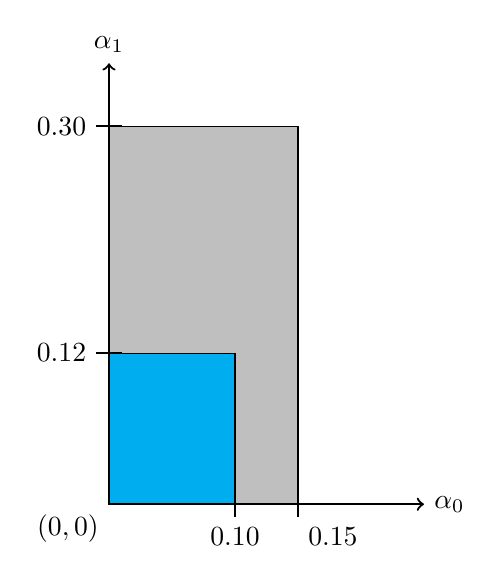
\begin{tikzpicture}[scale=16]
          \draw [fill = lightgray] (0,0) rectangle (0.15, 0.3);
          \draw [fill = cyan] (0,0) rectangle (0.10, 0.12);
          \draw [thick, <->] (0,0.35)
          node[above] {$\alpha_1$} -- (0,0) 
          node [below left] {$(0,0)$} -- (0.25,0) 
          node [right] {$\alpha_0$};
          \draw [thick] (0.15,0.01) -- (0.15,-0.01) node [below right] {$0.15$}; 
          \draw [thick] (0.1,0.01) -- (0.1,-0.01) node [below] {$0.10$}; 
          \draw [thick] (0.01,0.3) -- (-0.01,0.3) node [left] {0.30}; 
          \draw [thick] (0.01,0.12) -- (-0.01,0.12) node [left] {0.12}; 
          \end{tikzpicture}
      \end{figure}
  \end{column}
\end{columns}
 
\end{frame}
%%%%%%%%%%%%%%%%%%%%%%%%%%%%%%%%%%%%%%
\begin{frame}
  \frametitle{Independence Assumption: $\varepsilon \perp T |(T^*,z)$}
  Define $F_{tk}(\tau) = \mathbb{P}(Y \leq \tau|T=t, z_k)$ and $F_k(\tau) = \mathbb{P}(Y \leq \tau|z_k)$

\begin{align*}
  \alpha_0 &\leq p_k \inf_\tau\left\{\left[\frac{F_{1k}(\tau)}{F_k(\tau)}\right] \wedge \left[\frac{1-F_{1k}(\tau)}{1 - F_k(\tau)} \right]\right\} \leq p_k \\ \\
  \alpha_1 &\leq (1 - p_k) \inf_\tau \left\{\left[\frac{F_{0k}(\tau)}{F_k(\tau)}\right] \wedge \left[\frac{1-F_{0k}(\tau)}{1 - F_k(\tau)} \right]\right\} \leq (1 - p_k) 
\end{align*}

\vspace{1em}
\alert{Bounds for $(\alpha_0, \alpha_1)$ do \emph{not} require $z$ to be a valid instrument!}
\end{frame}
%%%%%%%%%%%%%%%%%%%%%%%%%%%%%%%%%%%%%%
\begin{frame}
  \frametitle{Upper Bounds for Mis-Classification Rates}
  \framesubtitle{Returns to Schooling Example: Oreopoulos (2006)}
  \begin{figure}[h]
    \centering
    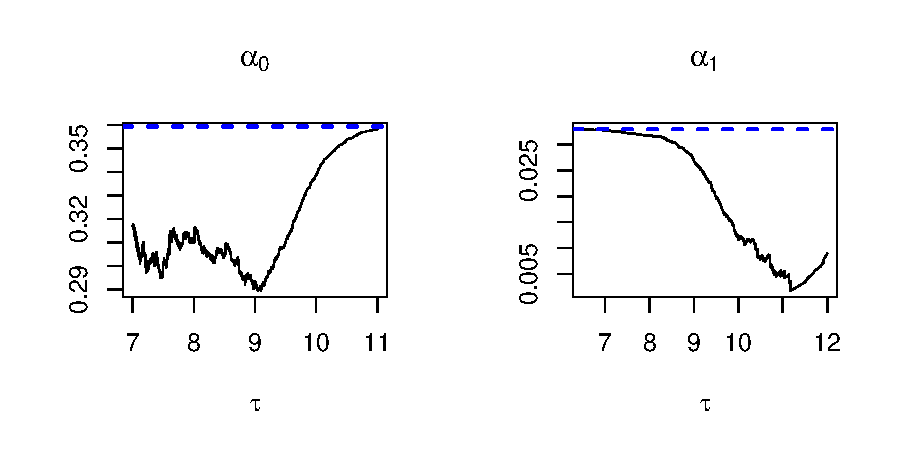
\includegraphics[width=\textwidth]{Oreo_CDFbounds}
  \end{figure}
\end{frame}
%%%%%%%%%%%%%%%%%%%%%%%%%%%%%%%%%%%%%%
\begin{frame}
  \frametitle{Sufficient Conditions To Identify $\alpha_0, \alpha_1$, and $\beta$}
  \small

  \begin{block}{Baseline Assumptions}
  \vspace{-1em}
    \begin{itemize}
      \item $\mathbb{E}[\varepsilon|z] =0$
      \item $\mathbb{E}[\varepsilon|T^*,T,z] = \mathbb{E}[\varepsilon|T^*,z]$
      \item $\alpha_0 = \mathbb{P}(T=1|T^*=0,z), \; \alpha_1 =\mathbb{P}(T=0|T^*=1, z), \; \alpha_0 + \alpha_1 < 1$
    \end{itemize}
  \end{block}

  \vspace{-1em}
  
  \begin{alertblock}{Strengthen IV Assumption}
  \vspace{-1em}
    \begin{itemize}
      \item $\mathbb{E}[\varepsilon^2|z] = \mathbb{E}[\varepsilon^2]$  
      \item $\mathbb{E}[\varepsilon^3|z] = \mathbb{E}[\varepsilon^3]$  
    \end{itemize}
  \end{alertblock}

  \vspace{-1em}
  \begin{alertblock}{Strengthen Measurement Error Assumption}
  \vspace{-1em}
    \begin{itemize}
      \item $\mathbb{E}[\varepsilon^2|T^*,T,z] = \mathbb{E}[\varepsilon^2|T^*,z]$  
      \item $\mathbb{E}[\varepsilon^3|T^*,T,z] = \mathbb{E}[\varepsilon^3|T^*,z]$  
    \end{itemize}

  \end{alertblock}

\end{frame}
%%%%%%%%%%%%%%%%%%%%%%%%%%%%%%%%%%%%%%
\begin{frame}
  \frametitle{First Moment Condition}
  \begin{block}{Assumptions}
    \begin{itemize}
      \item $\mathbb{E}[\varepsilon|z]=0$
      \item $\mathbb{E}[\varepsilon|T^*,T,z] =  \mathbb{E}[\varepsilon|T^*,z]$
      \item $\alpha_0 = \mathbb{P}(T = 1| T^* = 0, z)$ 
      \item  $\alpha_1 = \mathbb{P}(T = 0| T^* = 1, z)$ 
    \end{itemize}
  \end{block}

  \begin{block}{Moment Condition}
    \[\mbox{Cov}(y,z) - \left( \frac{\beta}{1 - \alpha_0 - \alpha_1} \right) \mbox{Cov}(T,z) = 0\]
  \end{block}

  \alert{MC \# 1 identifies $\beta/(1 - \alpha_0 - \alpha_1)$}
\end{frame}
%%%%%%%%%%%%%%%%%%%%%%%%%%%%%%%%%%%%%%
\begin{frame}
  \frametitle{Second Moment Condition}
  \begin{block}{Additional Assumptions}
    \begin{itemize}
      \item $\mathbb{E}[\varepsilon^2|z]=\mathbb{E}[\varepsilon^2]$
      \item $\mathbb{E}[\varepsilon^2|T^*,T,z] =  \mathbb{E}[\varepsilon|T^*,z]$
    \end{itemize}
  \end{block}

  \begin{block}{Moment Condition}
    \small
  \[\mbox{Cov}(y^2,z) - \frac{\beta}{1 - \alpha_0 - \alpha_1}\left\{2\mbox{Cov}(yT,z)- \beta \mbox{Cov}(T,z)\left( \frac{1 + \alpha_0 - \alpha_1}{1 - \alpha_0 - \alpha_1} \right)  \right\} = 0\]
  \end{block}

  \alert{Given MC \#1, MC \#2 identifies $(\alpha_1 - \alpha_0)$}
\end{frame}
%%%%%%%%%%%%%%%%%%%%%%%%%%%%%%%%%%%%%%
\begin{frame}
  \frametitle{Third Moment Condition}
  \begin{block}{Additional Assumptions}
    \begin{itemize}
      \item $\mathbb{E}[\varepsilon^3|z]=\mathbb{E}[\varepsilon^2]$
      \item $\mathbb{E}[\varepsilon^3|T^*,T,z] =  \mathbb{E}[\varepsilon|T^*,z]$
    \end{itemize}
  \end{block}
  \begin{block}{Moment Condition}
\scriptsize
\begin{align*}
  \mbox{Cov}(y^3,z) - \left( \frac{\beta}{1 - \alpha_0 - \alpha_1} \right)\Bigg \{& \left. \beta^2\left[1 + \frac{6\alpha_0(1 - \alpha_1)}{(1 - \alpha_0 - \alpha_1)^2} \right] \mbox{Cov}(T,z)\right.\\ & \left. - 3\beta\left[ \frac{1 - (\alpha_1 - \alpha_0)}{1 - \alpha_0 - \alpha_1} \right] \mbox{Cov}(yT,z) + 3\mbox{Cov}(y^2T,z) \right\} = 0
\end{align*}
\end{block}
\normalsize
\end{frame}
%%%%%%%%%%%%%%%%%%%%%%%%%%%%%%%%%%%%%%
\begin{frame}
  \frametitle{Sketch of Identification Argument}
  \alert{Very tedious algebra\ldots}
  \begin{enumerate}
    \item Use 1st MC to eliminate $\beta/(1 - \alpha_0 - \alpha_1)$ from others
    \item Use 2nd MC to solve for $\alpha_1$ in terms of $\alpha_0$ 
    \item 3rd MC becomes a quadratic in $(1-\alpha_1)$ and observables only.
    \item The quadratic always has two real roots: $(1 - \alpha_1)$ and $\alpha_0$.
    \item To tell which root is which, use $\alpha_0 + \alpha_1 < 1$.
    \item Calculate $\alpha_0 + \alpha_1$ and substitute into 1st MC to obtain $\beta$.
  \end{enumerate}

  \vspace{1em}
  \alert{Unfortunately, identification of $\alpha_0, \alpha_1$ fails if $\beta = 0$\ldots}
\end{frame}
%%%%%%%%%%%%%%%%%%%%%%%%%%%%%%%%%%%%%%
\begin{frame}
  \frametitle{Simple Special Case: $\alpha_0 = 0$}
  \begin{align*}
    \mbox{Cov}(y,z) - \left( \frac{\beta}{1 - \alpha_0} \right) \mbox{Cov}(T,z) &= 0\\
  \mbox{Cov}(y^2,z) - \frac{\beta}{1 - \alpha_0}\left\{2\mbox{Cov}(yT,z)- \beta \mbox{Cov}(T,z)\right\} &= 0
  \end{align*}

  \vspace{1em}
  \[
    \alert{\beta = \frac{2\mbox{Cov}(yT,z)}{\mbox{Cov}(T,z)} - \frac{\mbox{Cov}(y^2,z)}{\mbox{Cov}(y,z)}}
  \]

\end{frame}
%%%%%%%%%%%%%%%%%%%%%%%%%%%%%%%%%%%%%%

%%%%%%%%%%%%%%%%%%%%%%%%%%%%%%%%%%%%%%
%\begin{frame}
%  \frametitle{Empirical Illustration: Schooling and Test Scores}
%\framesubtitle{Burde \& Linden (2013, AEJ Applied)}
%  RCT in Afghanistan: 32 villages divided into 11 clusters. Randomly choose 6 and build a school in each village of these clusters ($N = 1468$).
%
%\begin{itemize}
%  \item $y$ -- Child's score on math and language test 
%  \item $T^*$ -- Child's true school attendance
%  \item $T$ -- Parent's report of child's school attendance
%  \item $\mathbf{x}$ -- Child and household characteristics
%  \item $z$ -- School built in village
%\end{itemize}
%\end{frame}
%%%%%%%%%%%%%%%%%%%%%%%%%%%%%%%%%%%%%%%%
%\begin{frame}
%  \frametitle{Empirical Illustration: Schooling and Test Scores}
%\framesubtitle{Burde \& Linden (2013, AEJ Applied)}
%\begin{figure}[h]
%  \scriptsize
%  \begingroup
%  \tikzset{every picture/.style={scale=0.53}}
%  \centering
%  % Created by tikzDevice version 0.8.1 on 2015-11-17 20:04:01
% !TEX encoding = UTF-8 Unicode
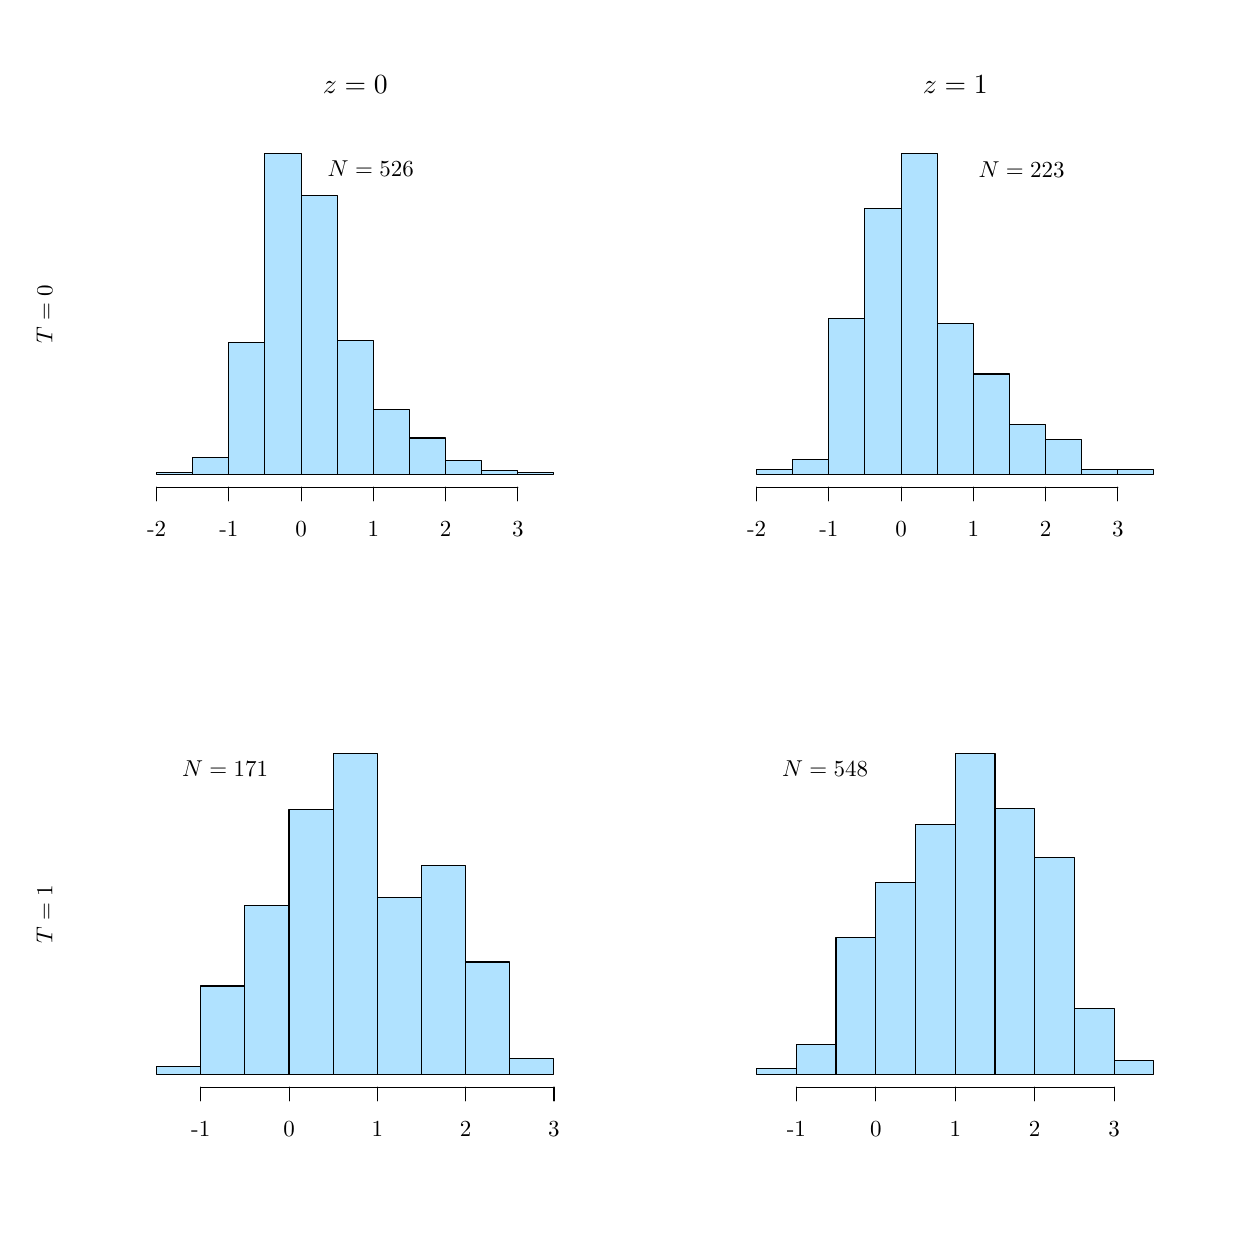
\begin{tikzpicture}[x=1pt,y=1pt]
\definecolor{fillColor}{RGB}{255,255,255}
\path[use as bounding box,fill=fillColor,fill opacity=0.00] (0,0) rectangle (433.62,433.62);
\begin{scope}
\path[clip] (  0.00,  0.00) rectangle (433.62,433.62);
\definecolor{drawColor}{RGB}{0,0,0}

\path[draw=drawColor,line width= 0.4pt,line join=round,line cap=round] ( 46.59,267.61) -- (177.11,267.61);

\path[draw=drawColor,line width= 0.4pt,line join=round,line cap=round] ( 46.59,267.61) -- ( 46.59,262.63);

\path[draw=drawColor,line width= 0.4pt,line join=round,line cap=round] ( 72.70,267.61) -- ( 72.70,262.63);

\path[draw=drawColor,line width= 0.4pt,line join=round,line cap=round] ( 98.80,267.61) -- ( 98.80,262.63);

\path[draw=drawColor,line width= 0.4pt,line join=round,line cap=round] (124.90,267.61) -- (124.90,262.63);

\path[draw=drawColor,line width= 0.4pt,line join=round,line cap=round] (151.01,267.61) -- (151.01,262.63);

\path[draw=drawColor,line width= 0.4pt,line join=round,line cap=round] (177.11,267.61) -- (177.11,262.63);

\node[text=drawColor,anchor=base,inner sep=0pt, outer sep=0pt, scale=  0.83] at ( 46.59,249.68) {-2};

\node[text=drawColor,anchor=base,inner sep=0pt, outer sep=0pt, scale=  0.83] at ( 72.70,249.68) {-1};

\node[text=drawColor,anchor=base,inner sep=0pt, outer sep=0pt, scale=  0.83] at ( 98.80,249.68) {0};

\node[text=drawColor,anchor=base,inner sep=0pt, outer sep=0pt, scale=  0.83] at (124.90,249.68) {1};

\node[text=drawColor,anchor=base,inner sep=0pt, outer sep=0pt, scale=  0.83] at (151.01,249.68) {2};

\node[text=drawColor,anchor=base,inner sep=0pt, outer sep=0pt, scale=  0.83] at (177.11,249.68) {3};
\end{scope}
\begin{scope}
\path[clip] (  0.00,216.81) rectangle (216.81,433.62);
\definecolor{drawColor}{RGB}{0,0,0}

\node[text=drawColor,anchor=base,inner sep=0pt, outer sep=0pt, scale=  1.00] at (118.36,409.77) {\bfseries $z = 0$};

\node[text=drawColor,rotate= 90.00,anchor=base,inner sep=0pt, outer sep=0pt, scale=  0.83] at (  8.96,330.19) {$T = 0$};
\end{scope}
\begin{scope}
\path[clip] ( 40.84,267.61) rectangle (195.89,392.78);
\definecolor{drawColor}{RGB}{0,0,0}
\definecolor{fillColor}{RGB}{176,226,255}

\path[draw=drawColor,line width= 0.4pt,line join=round,line cap=round,fill=fillColor] ( 46.58,272.24) rectangle ( 59.63,272.93);

\path[draw=drawColor,line width= 0.4pt,line join=round,line cap=round,fill=fillColor] ( 59.63,272.24) rectangle ( 72.68,278.45);

\path[draw=drawColor,line width= 0.4pt,line join=round,line cap=round,fill=fillColor] ( 72.68,272.24) rectangle ( 85.73,319.85);

\path[draw=drawColor,line width= 0.4pt,line join=round,line cap=round,fill=fillColor] ( 85.73,272.24) rectangle ( 98.79,388.15);

\path[draw=drawColor,line width= 0.4pt,line join=round,line cap=round,fill=fillColor] ( 98.79,272.24) rectangle (111.84,372.97);

\path[draw=drawColor,line width= 0.4pt,line join=round,line cap=round,fill=fillColor] (111.84,272.24) rectangle (124.89,320.54);

\path[draw=drawColor,line width= 0.4pt,line join=round,line cap=round,fill=fillColor] (124.89,272.24) rectangle (137.94,295.70);

\path[draw=drawColor,line width= 0.4pt,line join=round,line cap=round,fill=fillColor] (137.94,272.24) rectangle (151.00,285.35);

\path[draw=drawColor,line width= 0.4pt,line join=round,line cap=round,fill=fillColor] (151.00,272.24) rectangle (164.05,277.07);

\path[draw=drawColor,line width= 0.4pt,line join=round,line cap=round,fill=fillColor] (164.05,272.24) rectangle (177.10,273.62);

\path[draw=drawColor,line width= 0.4pt,line join=round,line cap=round,fill=fillColor] (177.10,272.24) rectangle (190.15,272.93);

\node[text=drawColor,anchor=base west,inner sep=0pt, outer sep=0pt, scale=  0.83] at (108.42,379.97) {$N=526$};
\end{scope}
\begin{scope}
\path[clip] (  0.00,  0.00) rectangle (433.62,433.62);
\definecolor{drawColor}{RGB}{0,0,0}

\path[draw=drawColor,line width= 0.4pt,line join=round,line cap=round] (263.40,267.61) -- (393.92,267.61);

\path[draw=drawColor,line width= 0.4pt,line join=round,line cap=round] (263.40,267.61) -- (263.40,262.63);

\path[draw=drawColor,line width= 0.4pt,line join=round,line cap=round] (289.51,267.61) -- (289.51,262.63);

\path[draw=drawColor,line width= 0.4pt,line join=round,line cap=round] (315.61,267.61) -- (315.61,262.63);

\path[draw=drawColor,line width= 0.4pt,line join=round,line cap=round] (341.71,267.61) -- (341.71,262.63);

\path[draw=drawColor,line width= 0.4pt,line join=round,line cap=round] (367.82,267.61) -- (367.82,262.63);

\path[draw=drawColor,line width= 0.4pt,line join=round,line cap=round] (393.92,267.61) -- (393.92,262.63);

\node[text=drawColor,anchor=base,inner sep=0pt, outer sep=0pt, scale=  0.83] at (263.40,249.68) {-2};

\node[text=drawColor,anchor=base,inner sep=0pt, outer sep=0pt, scale=  0.83] at (289.51,249.68) {-1};

\node[text=drawColor,anchor=base,inner sep=0pt, outer sep=0pt, scale=  0.83] at (315.61,249.68) {0};

\node[text=drawColor,anchor=base,inner sep=0pt, outer sep=0pt, scale=  0.83] at (341.71,249.68) {1};

\node[text=drawColor,anchor=base,inner sep=0pt, outer sep=0pt, scale=  0.83] at (367.82,249.68) {2};

\node[text=drawColor,anchor=base,inner sep=0pt, outer sep=0pt, scale=  0.83] at (393.92,249.68) {3};
\end{scope}
\begin{scope}
\path[clip] (216.81,216.81) rectangle (433.62,433.62);
\definecolor{drawColor}{RGB}{0,0,0}

\node[text=drawColor,anchor=base,inner sep=0pt, outer sep=0pt, scale=  1.00] at (335.17,409.77) {\bfseries $z = 1$};
\end{scope}
\begin{scope}
\path[clip] (257.65,267.61) rectangle (412.70,392.78);
\definecolor{drawColor}{RGB}{0,0,0}
\definecolor{fillColor}{RGB}{176,226,255}

\path[draw=drawColor,line width= 0.4pt,line join=round,line cap=round,fill=fillColor] (263.39,272.24) rectangle (276.44,274.05);

\path[draw=drawColor,line width= 0.4pt,line join=round,line cap=round,fill=fillColor] (276.44,272.24) rectangle (289.49,277.68);

\path[draw=drawColor,line width= 0.4pt,line join=round,line cap=round,fill=fillColor] (289.49,272.24) rectangle (302.54,328.38);

\path[draw=drawColor,line width= 0.4pt,line join=round,line cap=round,fill=fillColor] (302.54,272.24) rectangle (315.60,368.23);

\path[draw=drawColor,line width= 0.4pt,line join=round,line cap=round,fill=fillColor] (315.60,272.24) rectangle (328.65,388.15);

\path[draw=drawColor,line width= 0.4pt,line join=round,line cap=round,fill=fillColor] (328.65,272.24) rectangle (341.70,326.57);

\path[draw=drawColor,line width= 0.4pt,line join=round,line cap=round,fill=fillColor] (341.70,272.24) rectangle (354.75,308.46);

\path[draw=drawColor,line width= 0.4pt,line join=round,line cap=round,fill=fillColor] (354.75,272.24) rectangle (367.81,290.35);

\path[draw=drawColor,line width= 0.4pt,line join=round,line cap=round,fill=fillColor] (367.81,272.24) rectangle (380.86,284.92);

\path[draw=drawColor,line width= 0.4pt,line join=round,line cap=round,fill=fillColor] (380.86,272.24) rectangle (393.91,274.05);

\path[draw=drawColor,line width= 0.4pt,line join=round,line cap=round,fill=fillColor] (393.91,272.24) rectangle (406.96,274.05);

\node[text=drawColor,anchor=base west,inner sep=0pt, outer sep=0pt, scale=  0.83] at (343.60,379.49) {$N=223$};
\end{scope}
\begin{scope}
\path[clip] (  0.00,  0.00) rectangle (433.62,433.62);
\definecolor{drawColor}{RGB}{0,0,0}

\path[draw=drawColor,line width= 0.4pt,line join=round,line cap=round] ( 62.55, 50.80) -- (190.17, 50.80);

\path[draw=drawColor,line width= 0.4pt,line join=round,line cap=round] ( 62.55, 50.80) -- ( 62.55, 45.82);

\path[draw=drawColor,line width= 0.4pt,line join=round,line cap=round] ( 94.45, 50.80) -- ( 94.45, 45.82);

\path[draw=drawColor,line width= 0.4pt,line join=round,line cap=round] (126.36, 50.80) -- (126.36, 45.82);

\path[draw=drawColor,line width= 0.4pt,line join=round,line cap=round] (158.26, 50.80) -- (158.26, 45.82);

\path[draw=drawColor,line width= 0.4pt,line join=round,line cap=round] (190.17, 50.80) -- (190.17, 45.82);

\node[text=drawColor,anchor=base,inner sep=0pt, outer sep=0pt, scale=  0.83] at ( 62.55, 32.87) {-1};

\node[text=drawColor,anchor=base,inner sep=0pt, outer sep=0pt, scale=  0.83] at ( 94.45, 32.87) {0};

\node[text=drawColor,anchor=base,inner sep=0pt, outer sep=0pt, scale=  0.83] at (126.36, 32.87) {1};

\node[text=drawColor,anchor=base,inner sep=0pt, outer sep=0pt, scale=  0.83] at (158.26, 32.87) {2};

\node[text=drawColor,anchor=base,inner sep=0pt, outer sep=0pt, scale=  0.83] at (190.17, 32.87) {3};
\end{scope}
\begin{scope}
\path[clip] (  0.00,  0.00) rectangle (216.81,216.81);
\definecolor{drawColor}{RGB}{0,0,0}

\node[text=drawColor,rotate= 90.00,anchor=base,inner sep=0pt, outer sep=0pt, scale=  0.83] at (  8.96,113.38) {$T = 1$};
\end{scope}
\begin{scope}
\path[clip] ( 40.84, 50.80) rectangle (195.89,175.97);
\definecolor{drawColor}{RGB}{0,0,0}
\definecolor{fillColor}{RGB}{176,226,255}

\path[draw=drawColor,line width= 0.4pt,line join=round,line cap=round,fill=fillColor] ( 46.58, 55.43) rectangle ( 62.53, 58.33);

\path[draw=drawColor,line width= 0.4pt,line join=round,line cap=round,fill=fillColor] ( 62.53, 55.43) rectangle ( 78.48, 87.31);

\path[draw=drawColor,line width= 0.4pt,line join=round,line cap=round,fill=fillColor] ( 78.48, 55.43) rectangle ( 94.44,116.28);

\path[draw=drawColor,line width= 0.4pt,line join=round,line cap=round,fill=fillColor] ( 94.44, 55.43) rectangle (110.39,151.05);

\path[draw=drawColor,line width= 0.4pt,line join=round,line cap=round,fill=fillColor] (110.39, 55.43) rectangle (126.34,171.34);

\path[draw=drawColor,line width= 0.4pt,line join=round,line cap=round,fill=fillColor] (126.34, 55.43) rectangle (142.29,119.18);

\path[draw=drawColor,line width= 0.4pt,line join=round,line cap=round,fill=fillColor] (142.29, 55.43) rectangle (158.25,130.77);

\path[draw=drawColor,line width= 0.4pt,line join=round,line cap=round,fill=fillColor] (158.25, 55.43) rectangle (174.20, 96.00);

\path[draw=drawColor,line width= 0.4pt,line join=round,line cap=round,fill=fillColor] (174.20, 55.43) rectangle (190.15, 61.23);

\node[text=drawColor,anchor=base west,inner sep=0pt, outer sep=0pt, scale=  0.83] at ( 55.78,163.16) {$N=171$};
\end{scope}
\begin{scope}
\path[clip] (  0.00,  0.00) rectangle (433.62,433.62);
\definecolor{drawColor}{RGB}{0,0,0}

\path[draw=drawColor,line width= 0.4pt,line join=round,line cap=round] (277.76, 50.80) -- (392.62, 50.80);

\path[draw=drawColor,line width= 0.4pt,line join=round,line cap=round] (277.76, 50.80) -- (277.76, 45.82);

\path[draw=drawColor,line width= 0.4pt,line join=round,line cap=round] (306.47, 50.80) -- (306.47, 45.82);

\path[draw=drawColor,line width= 0.4pt,line join=round,line cap=round] (335.19, 50.80) -- (335.19, 45.82);

\path[draw=drawColor,line width= 0.4pt,line join=round,line cap=round] (363.90, 50.80) -- (363.90, 45.82);

\path[draw=drawColor,line width= 0.4pt,line join=round,line cap=round] (392.62, 50.80) -- (392.62, 45.82);

\node[text=drawColor,anchor=base,inner sep=0pt, outer sep=0pt, scale=  0.83] at (277.76, 32.87) {-1};

\node[text=drawColor,anchor=base,inner sep=0pt, outer sep=0pt, scale=  0.83] at (306.47, 32.87) {0};

\node[text=drawColor,anchor=base,inner sep=0pt, outer sep=0pt, scale=  0.83] at (335.19, 32.87) {1};

\node[text=drawColor,anchor=base,inner sep=0pt, outer sep=0pt, scale=  0.83] at (363.90, 32.87) {2};

\node[text=drawColor,anchor=base,inner sep=0pt, outer sep=0pt, scale=  0.83] at (392.62, 32.87) {3};
\end{scope}
\begin{scope}
\path[clip] (257.65, 50.80) rectangle (412.70,175.97);
\definecolor{drawColor}{RGB}{0,0,0}
\definecolor{fillColor}{RGB}{176,226,255}

\path[draw=drawColor,line width= 0.4pt,line join=round,line cap=round,fill=fillColor] (263.39, 55.43) rectangle (277.75, 57.41);

\path[draw=drawColor,line width= 0.4pt,line join=round,line cap=round,fill=fillColor] (277.75, 55.43) rectangle (292.10, 66.33);

\path[draw=drawColor,line width= 0.4pt,line join=round,line cap=round,fill=fillColor] (292.10, 55.43) rectangle (306.46,104.96);

\path[draw=drawColor,line width= 0.4pt,line join=round,line cap=round,fill=fillColor] (306.46, 55.43) rectangle (320.82,124.78);

\path[draw=drawColor,line width= 0.4pt,line join=round,line cap=round,fill=fillColor] (320.82, 55.43) rectangle (335.17,145.58);

\path[draw=drawColor,line width= 0.4pt,line join=round,line cap=round,fill=fillColor] (335.17, 55.43) rectangle (349.53,171.34);

\path[draw=drawColor,line width= 0.4pt,line join=round,line cap=round,fill=fillColor] (349.53, 55.43) rectangle (363.89,151.52);

\path[draw=drawColor,line width= 0.4pt,line join=round,line cap=round,fill=fillColor] (363.89, 55.43) rectangle (378.25,133.69);

\path[draw=drawColor,line width= 0.4pt,line join=round,line cap=round,fill=fillColor] (378.25, 55.43) rectangle (392.60, 79.21);

\path[draw=drawColor,line width= 0.4pt,line join=round,line cap=round,fill=fillColor] (392.60, 55.43) rectangle (406.96, 60.39);

\node[text=drawColor,anchor=base west,inner sep=0pt, outer sep=0pt, scale=  0.83] at (272.59,163.16) {$N=548$};
\end{scope}
\end{tikzpicture}

%  \endgroup
%\end{figure}
%\end{frame}
%%%%%%%%%%%%%%%%%%%%%%%%%%%%%%%%%%%%%%%%
%\begin{frame}
%  \frametitle{Empirical Illustration: Schooling and Test Scores}
%\framesubtitle{Burde \& Linden (2013, AEJ Applied)}
%    \begin{columns}[c]
%    \column{.26\textwidth} 
%    $\widehat{\beta}_{OLS} = 0.88$
%
%    $\widehat{\beta}_{IV} = 1.27$
%
%    $\widehat{\alpha}_1 - \widehat{\alpha}_0 = 0.18$
%    \column{.73\textwidth}
%        \begin{figure}[h]
%          \scriptsize
%          \begingroup
%          \tikzset{every picture/.style={scale=0.53}}
%          \centering
%          % Created by tikzDevice version 0.8.1 on 2015-11-17 20:19:21
% !TEX encoding = UTF-8 Unicode
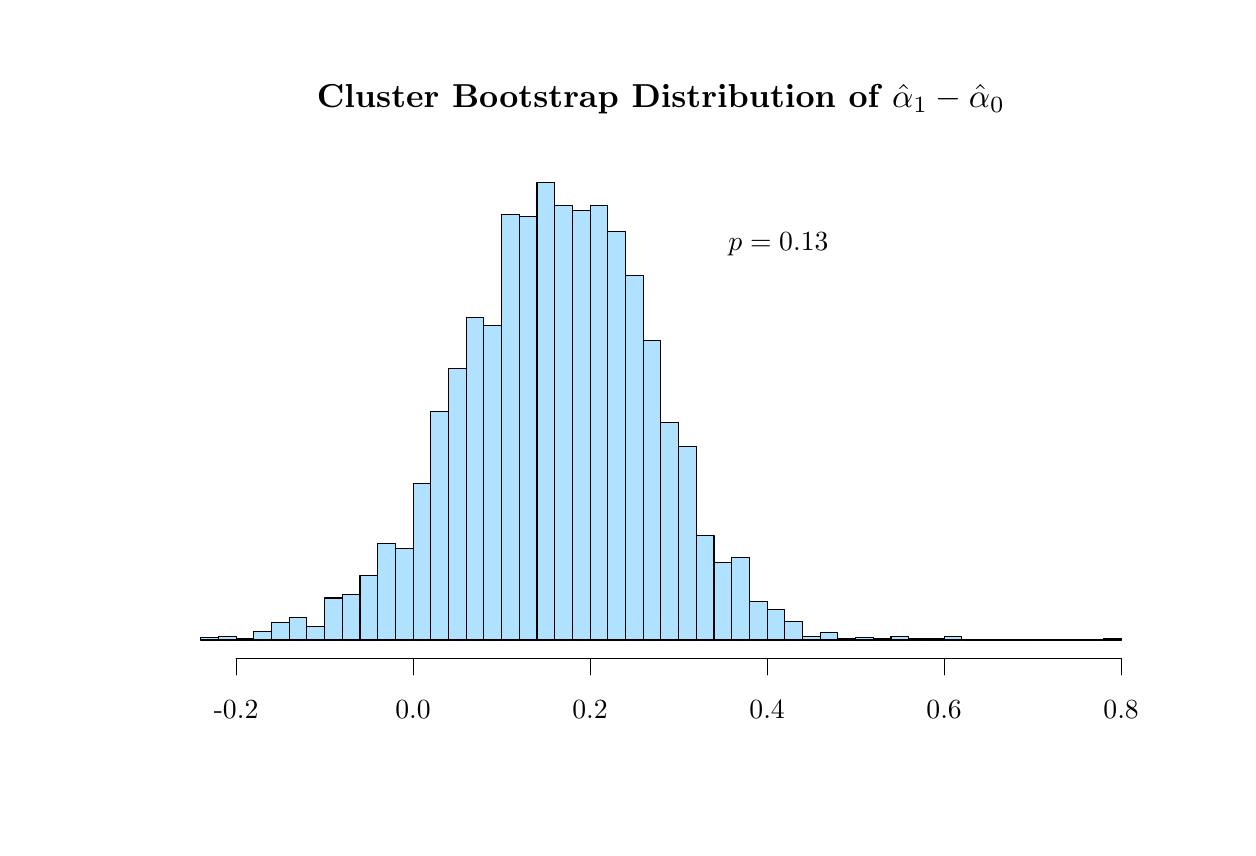
\begin{tikzpicture}[x=1pt,y=1pt]
\definecolor{fillColor}{RGB}{255,255,255}
\path[use as bounding box,fill=fillColor,fill opacity=0.00] (0,0) rectangle (433.62,289.08);
\begin{scope}
\path[clip] (  0.00,  0.00) rectangle (433.62,289.08);
\definecolor{drawColor}{RGB}{0,0,0}

\path[draw=drawColor,line width= 0.4pt,line join=round,line cap=round] ( 75.30, 61.20) -- (395.12, 61.20);

\path[draw=drawColor,line width= 0.4pt,line join=round,line cap=round] ( 75.30, 61.20) -- ( 75.30, 55.20);

\path[draw=drawColor,line width= 0.4pt,line join=round,line cap=round] (139.27, 61.20) -- (139.27, 55.20);

\path[draw=drawColor,line width= 0.4pt,line join=round,line cap=round] (203.23, 61.20) -- (203.23, 55.20);

\path[draw=drawColor,line width= 0.4pt,line join=round,line cap=round] (267.19, 61.20) -- (267.19, 55.20);

\path[draw=drawColor,line width= 0.4pt,line join=round,line cap=round] (331.16, 61.20) -- (331.16, 55.20);

\path[draw=drawColor,line width= 0.4pt,line join=round,line cap=round] (395.12, 61.20) -- (395.12, 55.20);

\node[text=drawColor,anchor=base,inner sep=0pt, outer sep=0pt, scale=  1.00] at ( 75.30, 39.60) {-0.2};

\node[text=drawColor,anchor=base,inner sep=0pt, outer sep=0pt, scale=  1.00] at (139.27, 39.60) {0.0};

\node[text=drawColor,anchor=base,inner sep=0pt, outer sep=0pt, scale=  1.00] at (203.23, 39.60) {0.2};

\node[text=drawColor,anchor=base,inner sep=0pt, outer sep=0pt, scale=  1.00] at (267.19, 39.60) {0.4};

\node[text=drawColor,anchor=base,inner sep=0pt, outer sep=0pt, scale=  1.00] at (331.16, 39.60) {0.6};

\node[text=drawColor,anchor=base,inner sep=0pt, outer sep=0pt, scale=  1.00] at (395.12, 39.60) {0.8};
\end{scope}
\begin{scope}
\path[clip] (  0.00,  0.00) rectangle (433.62,289.08);
\definecolor{drawColor}{RGB}{0,0,0}

\node[text=drawColor,anchor=base,inner sep=0pt, outer sep=0pt, scale=  1.20] at (228.81,260.34) {\bfseries Cluster Bootstrap Distribution of $\hat{\alpha}_1 - \hat{\alpha}_0$};
\end{scope}
\begin{scope}
\path[clip] ( 49.20, 61.20) rectangle (408.42,239.88);
\definecolor{drawColor}{RGB}{0,0,0}
\definecolor{fillColor}{RGB}{176,226,255}

\path[draw=drawColor,line width= 0.4pt,line join=round,line cap=round,fill=fillColor] ( 62.50, 67.82) rectangle ( 68.90, 68.71);

\path[draw=drawColor,line width= 0.4pt,line join=round,line cap=round,fill=fillColor] ( 68.90, 67.82) rectangle ( 75.30, 69.16);

\path[draw=drawColor,line width= 0.4pt,line join=round,line cap=round,fill=fillColor] ( 75.30, 67.82) rectangle ( 81.69, 68.26);

\path[draw=drawColor,line width= 0.4pt,line join=round,line cap=round,fill=fillColor] ( 81.69, 67.82) rectangle ( 88.09, 70.94);

\path[draw=drawColor,line width= 0.4pt,line join=round,line cap=round,fill=fillColor] ( 88.09, 67.82) rectangle ( 94.49, 74.06);

\path[draw=drawColor,line width= 0.4pt,line join=round,line cap=round,fill=fillColor] ( 94.49, 67.82) rectangle (100.88, 75.84);

\path[draw=drawColor,line width= 0.4pt,line join=round,line cap=round,fill=fillColor] (100.88, 67.82) rectangle (107.28, 72.72);

\path[draw=drawColor,line width= 0.4pt,line join=round,line cap=round,fill=fillColor] (107.28, 67.82) rectangle (113.68, 82.98);

\path[draw=drawColor,line width= 0.4pt,line join=round,line cap=round,fill=fillColor] (113.68, 67.82) rectangle (120.07, 84.32);

\path[draw=drawColor,line width= 0.4pt,line join=round,line cap=round,fill=fillColor] (120.07, 67.82) rectangle (126.47, 91.01);

\path[draw=drawColor,line width= 0.4pt,line join=round,line cap=round,fill=fillColor] (126.47, 67.82) rectangle (132.86,102.60);

\path[draw=drawColor,line width= 0.4pt,line join=round,line cap=round,fill=fillColor] (132.86, 67.82) rectangle (139.26,100.82);

\path[draw=drawColor,line width= 0.4pt,line join=round,line cap=round,fill=fillColor] (139.26, 67.82) rectangle (145.66,124.45);

\path[draw=drawColor,line width= 0.4pt,line join=round,line cap=round,fill=fillColor] (145.66, 67.82) rectangle (152.05,150.32);

\path[draw=drawColor,line width= 0.4pt,line join=round,line cap=round,fill=fillColor] (152.05, 67.82) rectangle (158.45,165.92);

\path[draw=drawColor,line width= 0.4pt,line join=round,line cap=round,fill=fillColor] (158.45, 67.82) rectangle (164.85,184.21);

\path[draw=drawColor,line width= 0.4pt,line join=round,line cap=round,fill=fillColor] (164.85, 67.82) rectangle (171.24,181.53);

\path[draw=drawColor,line width= 0.4pt,line join=round,line cap=round,fill=fillColor] (171.24, 67.82) rectangle (177.64,221.67);

\path[draw=drawColor,line width= 0.4pt,line join=round,line cap=round,fill=fillColor] (177.64, 67.82) rectangle (184.04,220.78);

\path[draw=drawColor,line width= 0.4pt,line join=round,line cap=round,fill=fillColor] (184.04, 67.82) rectangle (190.43,233.26);

\path[draw=drawColor,line width= 0.4pt,line join=round,line cap=round,fill=fillColor] (190.43, 67.82) rectangle (196.83,224.79);

\path[draw=drawColor,line width= 0.4pt,line join=round,line cap=round,fill=fillColor] (196.83, 67.82) rectangle (203.22,223.01);

\path[draw=drawColor,line width= 0.4pt,line join=round,line cap=round,fill=fillColor] (203.22, 67.82) rectangle (209.62,224.79);

\path[draw=drawColor,line width= 0.4pt,line join=round,line cap=round,fill=fillColor] (209.62, 67.82) rectangle (216.02,215.42);

\path[draw=drawColor,line width= 0.4pt,line join=round,line cap=round,fill=fillColor] (216.02, 67.82) rectangle (222.41,199.37);

\path[draw=drawColor,line width= 0.4pt,line join=round,line cap=round,fill=fillColor] (222.41, 67.82) rectangle (228.81,176.18);

\path[draw=drawColor,line width= 0.4pt,line join=round,line cap=round,fill=fillColor] (228.81, 67.82) rectangle (235.21,146.30);

\path[draw=drawColor,line width= 0.4pt,line join=round,line cap=round,fill=fillColor] (235.21, 67.82) rectangle (241.60,137.83);

\path[draw=drawColor,line width= 0.4pt,line join=round,line cap=round,fill=fillColor] (241.60, 67.82) rectangle (248.00,105.72);

\path[draw=drawColor,line width= 0.4pt,line join=round,line cap=round,fill=fillColor] (248.00, 67.82) rectangle (254.40, 95.91);

\path[draw=drawColor,line width= 0.4pt,line join=round,line cap=round,fill=fillColor] (254.40, 67.82) rectangle (260.79, 97.70);

\path[draw=drawColor,line width= 0.4pt,line join=round,line cap=round,fill=fillColor] (260.79, 67.82) rectangle (267.19, 81.64);

\path[draw=drawColor,line width= 0.4pt,line join=round,line cap=round,fill=fillColor] (267.19, 67.82) rectangle (273.58, 78.97);

\path[draw=drawColor,line width= 0.4pt,line join=round,line cap=round,fill=fillColor] (273.58, 67.82) rectangle (279.98, 74.51);

\path[draw=drawColor,line width= 0.4pt,line join=round,line cap=round,fill=fillColor] (279.98, 67.82) rectangle (286.38, 69.16);

\path[draw=drawColor,line width= 0.4pt,line join=round,line cap=round,fill=fillColor] (286.38, 67.82) rectangle (292.77, 70.49);

\path[draw=drawColor,line width= 0.4pt,line join=round,line cap=round,fill=fillColor] (292.77, 67.82) rectangle (299.17, 68.26);

\path[draw=drawColor,line width= 0.4pt,line join=round,line cap=round,fill=fillColor] (299.17, 67.82) rectangle (305.57, 68.71);

\path[draw=drawColor,line width= 0.4pt,line join=round,line cap=round,fill=fillColor] (305.57, 67.82) rectangle (311.96, 68.26);

\path[draw=drawColor,line width= 0.4pt,line join=round,line cap=round,fill=fillColor] (311.96, 67.82) rectangle (318.36, 69.16);

\path[draw=drawColor,line width= 0.4pt,line join=round,line cap=round,fill=fillColor] (318.36, 67.82) rectangle (324.76, 68.26);

\path[draw=drawColor,line width= 0.4pt,line join=round,line cap=round,fill=fillColor] (324.76, 67.82) rectangle (331.15, 68.26);

\path[draw=drawColor,line width= 0.4pt,line join=round,line cap=round,fill=fillColor] (331.15, 67.82) rectangle (337.55, 69.16);

\path[draw=drawColor,line width= 0.4pt,line join=round,line cap=round,fill=fillColor] (337.55, 67.82) rectangle (343.94, 67.82);

\path[draw=drawColor,line width= 0.4pt,line join=round,line cap=round,fill=fillColor] (343.94, 67.82) rectangle (350.34, 67.82);

\path[draw=drawColor,line width= 0.4pt,line join=round,line cap=round,fill=fillColor] (350.34, 67.82) rectangle (356.74, 67.82);

\path[draw=drawColor,line width= 0.4pt,line join=round,line cap=round,fill=fillColor] (356.74, 67.82) rectangle (363.13, 67.82);

\path[draw=drawColor,line width= 0.4pt,line join=round,line cap=round,fill=fillColor] (363.13, 67.82) rectangle (369.53, 67.82);

\path[draw=drawColor,line width= 0.4pt,line join=round,line cap=round,fill=fillColor] (369.53, 67.82) rectangle (375.93, 67.82);

\path[draw=drawColor,line width= 0.4pt,line join=round,line cap=round,fill=fillColor] (375.93, 67.82) rectangle (382.32, 67.82);

\path[draw=drawColor,line width= 0.4pt,line join=round,line cap=round,fill=fillColor] (382.32, 67.82) rectangle (388.72, 67.82);

\path[draw=drawColor,line width= 0.4pt,line join=round,line cap=round,fill=fillColor] (388.72, 67.82) rectangle (395.12, 68.26);

\node[text=drawColor,anchor=base west,inner sep=0pt, outer sep=0pt, scale=  1.00] at (253.21,208.45) {$p = 0.13$};
\end{scope}
\end{tikzpicture}

%          \endgroup
%        \end{figure}
%    \end{columns}
%\end{frame}
%
%%%%%%%%%%%%%%%%%%%%%%%%%%%%%%%%%%%%%%%
%\begin{frame}
%  \frametitle{Example: Vouchers for Private Schooling (PACES)}
%  \framesubtitle{Angrist et al.\ (2002, AER)}
%
%  Data from Colombia: vouchers to attend private school awarded by lottery to poor, primary school-aged children (N = 1577). 
%  
%
%\begin{itemize}
%  \item $y$ -- \# of grades repeated after lottery
%  \item $T^*$ -- Scholarship use 
%  \item $T$ -- Self-reported Scholarship use
%  \item $\mathbf{x}$ -- Demographic controls
%  \item $z$ -- Offered scholarship through lottery 
%\end{itemize}
%
%\alert{Authors raise concerns about the lottery in one of the two cities\ldots}
%\end{frame}
%
%%%%%%%%%%%%%%%%%%%%%%%%%%%%%%%%%%%%%%%%
%\begin{frame}
%  \frametitle{Example: Vouchers for Private Schooling (PACES)}
%  \framesubtitle{Overall: Mean = 0.19, SD = 0.45}
%\begin{figure}[h]
%  \scriptsize
%  \begingroup
%  \tikzset{every picture/.style={scale=0.53}}
%  \centering
%  \input{../../../sick-instruments/fig/AngristBettinger/hist.tex}
%  \endgroup
%\end{figure}
%\end{frame}
%%%%%%%%%%%%%%%%%%%%%%%%%%%%%%%%%%%%%%%%
%%%%%%%%%%%%%%%%%%%%%%%%%%%%%%%%%%%%
%\begin{frame}
%  \begin{center}
%    \Huge Simulation Study
%  \end{center}
%\end{frame}
%%%%%%%%%%%%%%%%%%%%%%%%%%%%%%%%%%%%%
\begin{frame}
  \frametitle{Simulation Example: $y = \beta T^* + \varepsilon$}
  \begin{block}{Errors}
      $(\varepsilon, \eta) \sim $ jointly normal, mean 0, variance 1, correlation 0.5.
  \end{block}
  \begin{block}{First-Stage}
      \begin{itemize}
        \item Half of subjects have $z=1$, the rest have $z=0$.
        \item $T^* = \mathbf{1}\left\{ \gamma_0 + \gamma_1 z + \eta > 0 \right\}$
        \item $\delta = \mathbb{P}(T^* = 0|z =1) = \mathbb{P}(T^*=1|z=0)$
          %\begin{itemize}
        %\item $\gamma_0 = \Phi^{-1}(\delta)$
        %\item $\gamma_1 = \Phi^{-1}(1-\delta) - \Phi(\delta)$   
      %\end{itemize}
      \end{itemize}
  \end{block}
  \vspace{-1em}


  \begin{block}{Mis-classification}
      \begin{itemize}
        \item Set $\alpha_0 = 0$ so $T^* = 0 \implies T=0$
        \item $T|T^*=1 \sim \mbox{Bernoulli}(1-\alpha_1)$
      \end{itemize}
  \end{block}
  
\end{frame}
%%%%%%%%%%%%%%%%%%%%%%%%%%%%%%%%%%%%%%
\begin{frame}[plain,c]

  \begin{figure}[h]
    \centering
    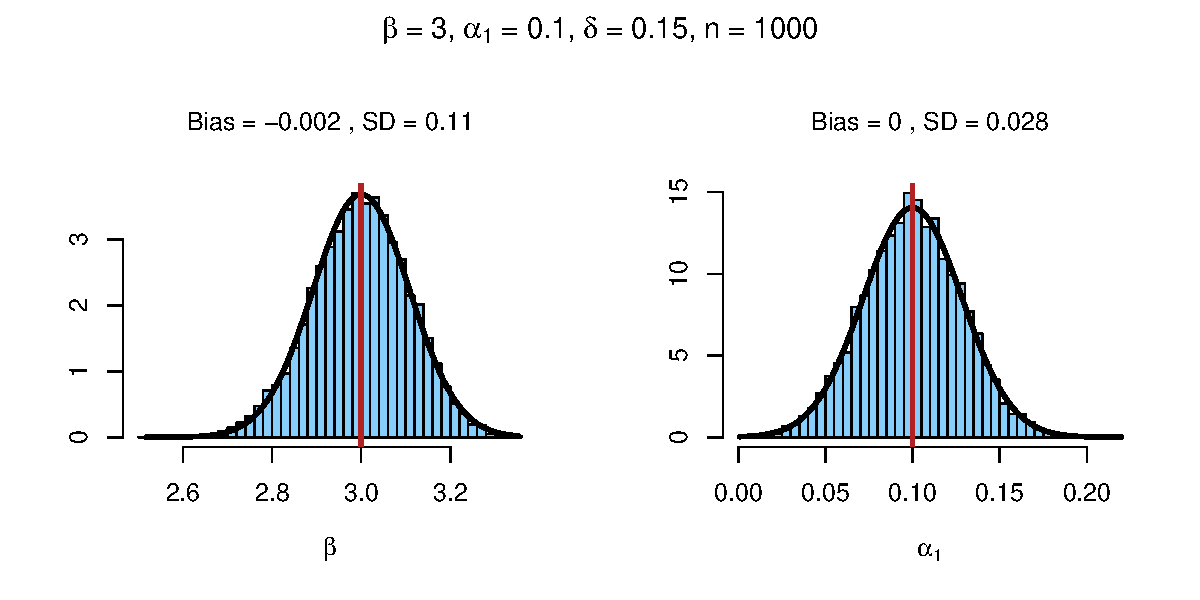
\includegraphics[width=\textwidth]{Rplot1}
  \end{figure}

\end{frame}
%%%%%%%%%%%%%%%%%%%%%%%%%%%%%%%%%%%%%%
\begin{frame}[plain,c]

  \begin{figure}[h]
    \centering
    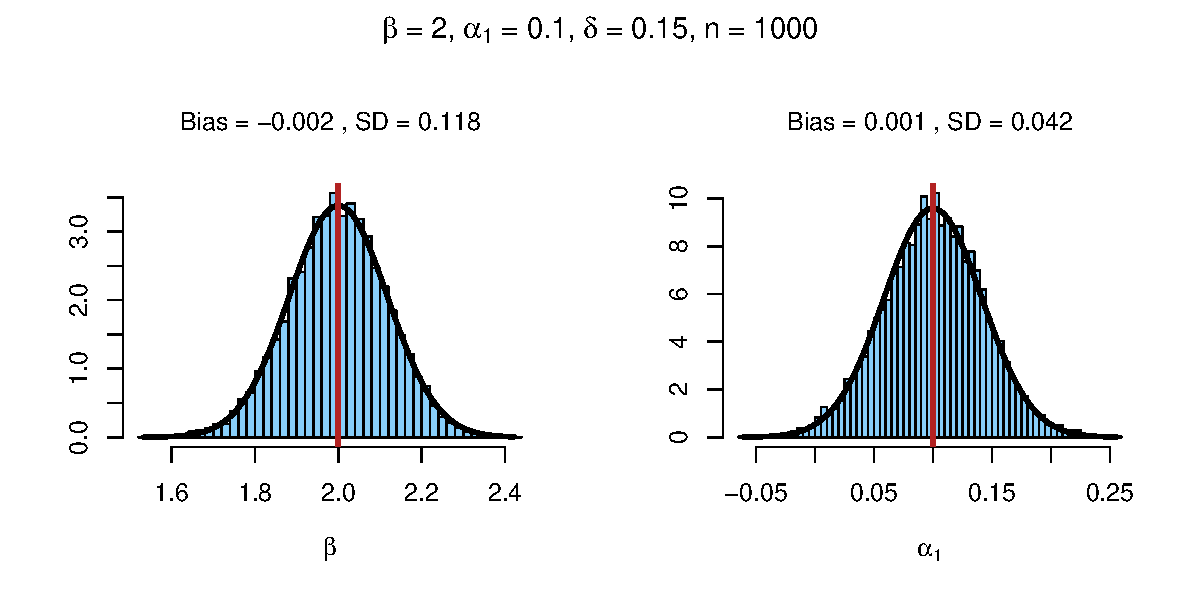
\includegraphics[width=\textwidth]{Rplot2}
  \end{figure}

\end{frame}
%%%%%%%%%%%%%%%%%%%%%%%%%%%%%%%%%%%%%%
\begin{frame}[plain,c]

  \begin{figure}[h]
    \centering
    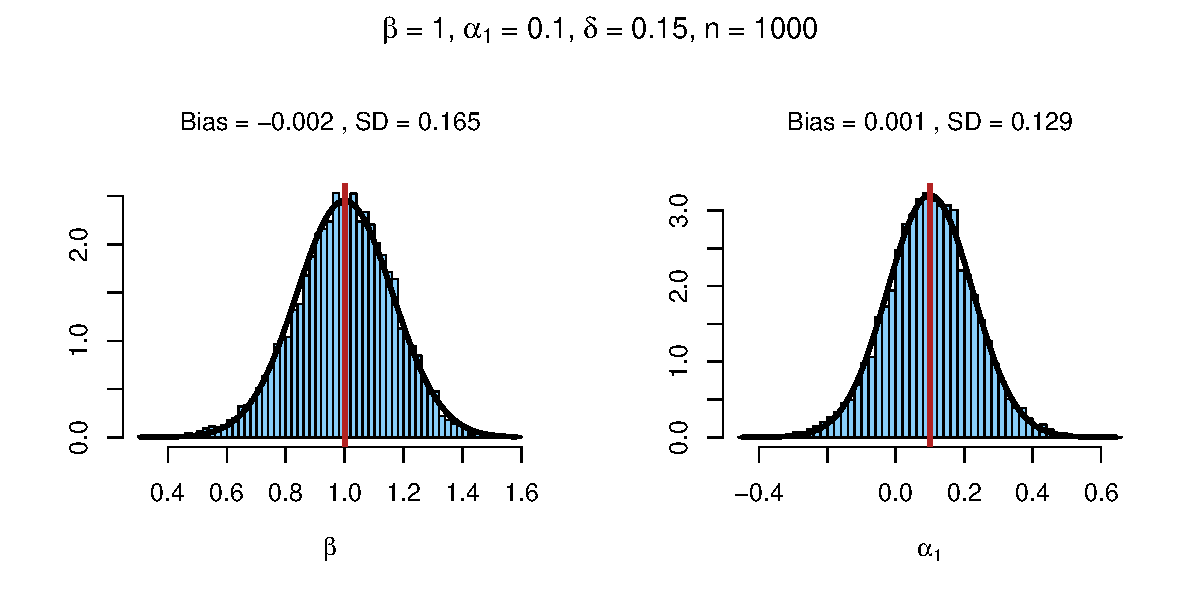
\includegraphics[width=\textwidth]{Rplot4}
  \end{figure}

\end{frame}
%%%%%%%%%%%%%%%%%%%%%%%%%%%%%%%%%%%%%%
\begin{frame}[plain,c]

  \begin{figure}[h]
    \centering
    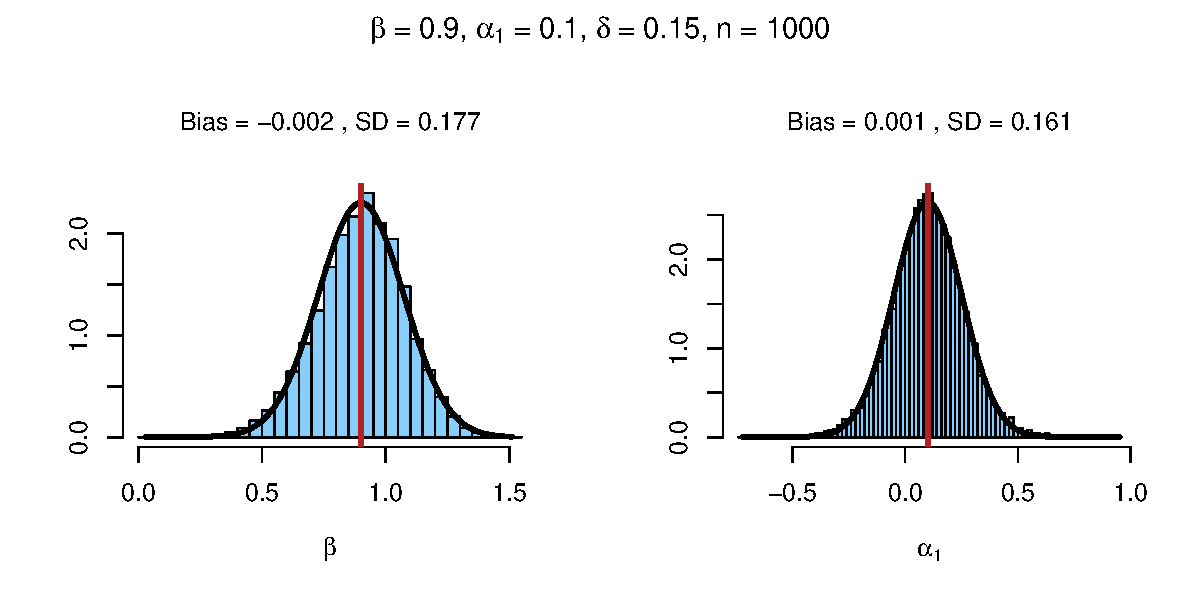
\includegraphics[width=\textwidth]{Rplot5}
  \end{figure}

\end{frame}
%%%%%%%%%%%%%%%%%%%%%%%%%%%%%%%%%%%%%%
\begin{frame}[plain,c]

  \begin{figure}[h]
    \centering
    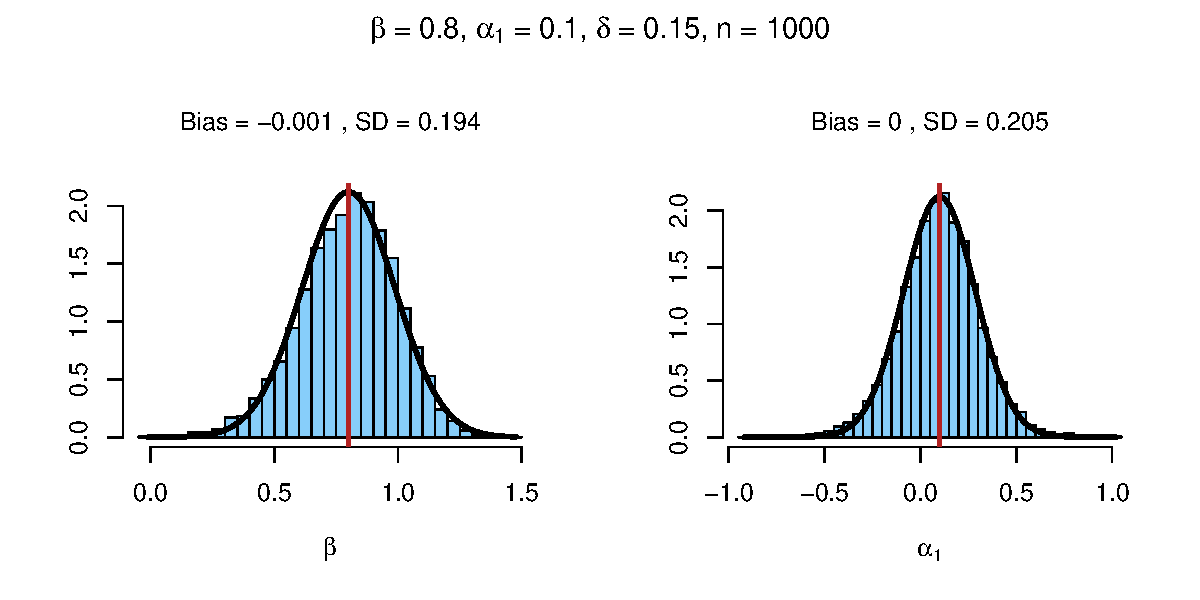
\includegraphics[width=\textwidth]{Rplot6}
  \end{figure}

\end{frame}
%%%%%%%%%%%%%%%%%%%%%%%%%%%%%%%%%%%%%%
\begin{frame}[plain,c]

  \begin{figure}[h]
    \centering
    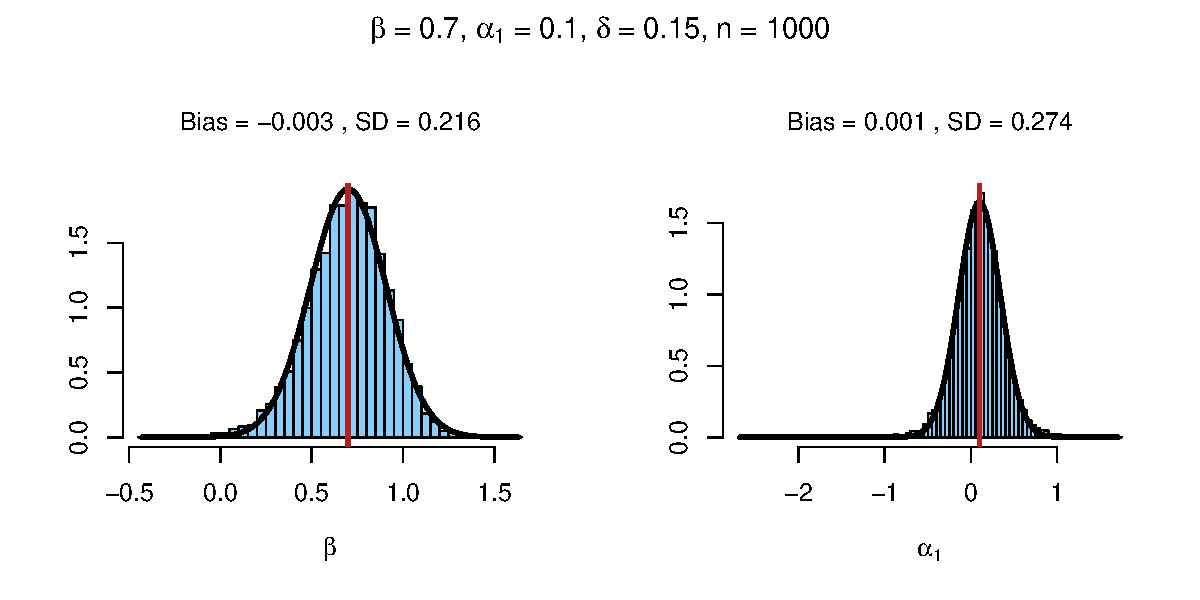
\includegraphics[width=\textwidth]{Rplot7}
  \end{figure}

\end{frame}
%%%%%%%%%%%%%%%%%%%%%%%%%%%%%%%%%%%%%%
\begin{frame}[plain,c]

  \begin{figure}[h]
    \centering
    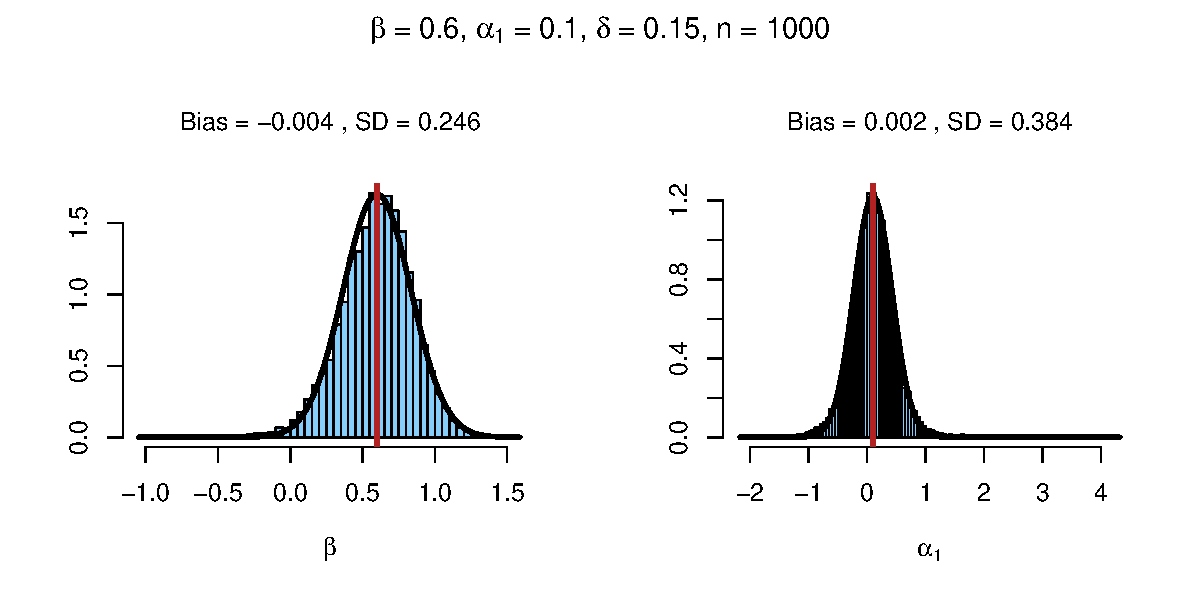
\includegraphics[width=\textwidth]{Rplot8}
  \end{figure}

\end{frame}
%%%%%%%%%%%%%%%%%%%%%%%%%%%%%%%%%%%%%%
\begin{frame}[plain,c]

  \begin{figure}[h]
    \centering
    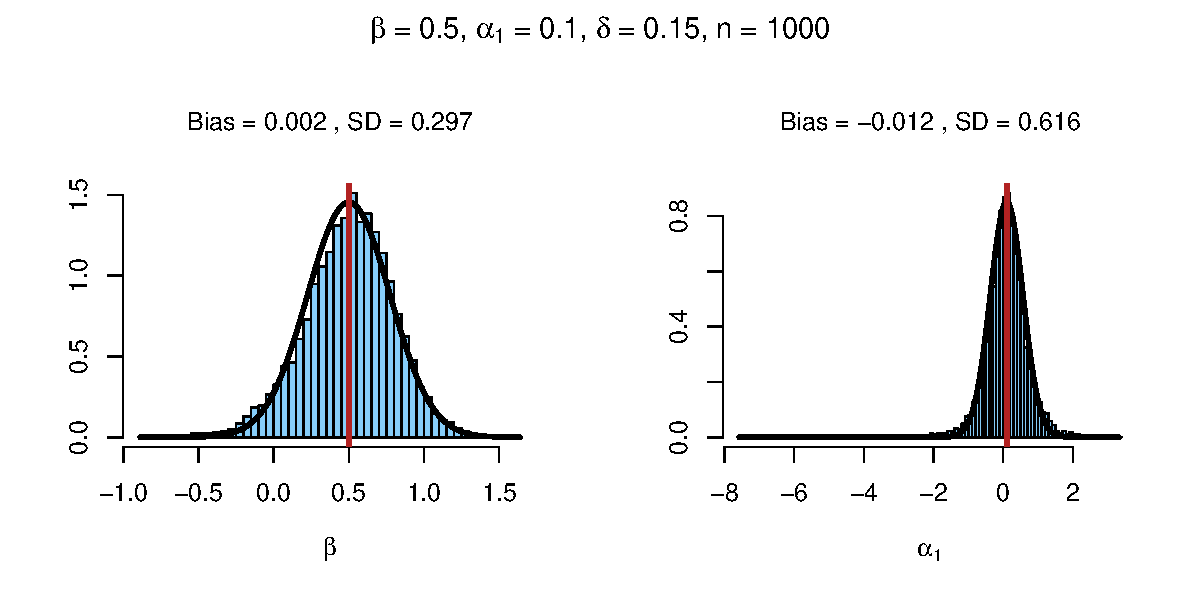
\includegraphics[width=\textwidth]{Rplot9}
  \end{figure}

\end{frame}
%%%%%%%%%%%%%%%%%%%%%%%%%%%%%%%%%%%%%%
\begin{frame}[plain,c]

  \begin{figure}[h]
    \centering
    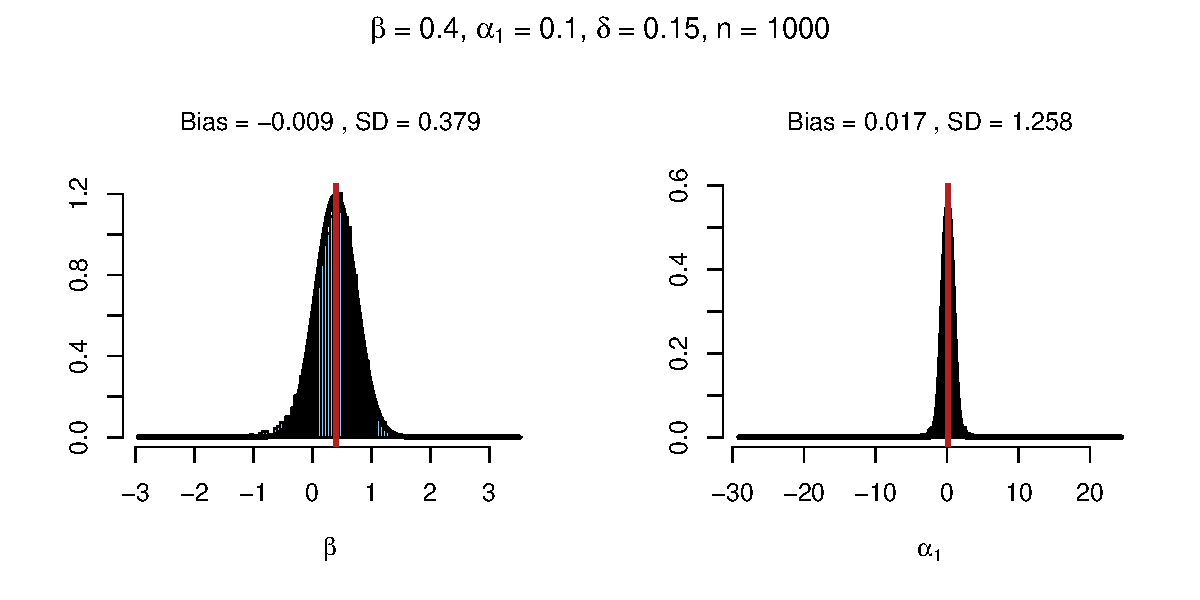
\includegraphics[width=\textwidth]{Rplot10}
  \end{figure}

\end{frame}
%%%%%%%%%%%%%%%%%%%%%%%%%%%%%%%%%%%%%%
\begin{frame}[plain,c]

  \begin{figure}[h]
    \centering
    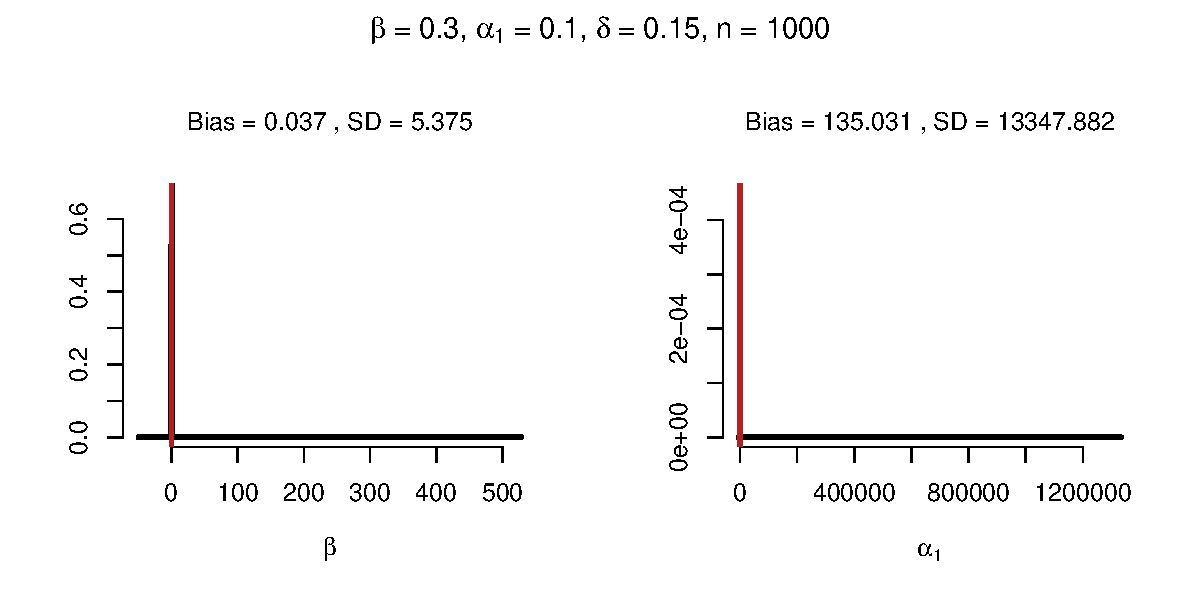
\includegraphics[width=\textwidth]{Rplot11}
  \end{figure}

\end{frame}
%%%%%%%%%%%%%%%%%%%%%%%%%%%%%%%%%%%%%%
\begin{frame}
  \frametitle{$(z \perp \varepsilon)$ and $(T\perp \varepsilon|T^*,z) \Rightarrow$ Continuum of MCs}

  \begin{block}{Characteristic Functions}
    \vspace{-1em}
\[
  e^{i\omega\beta}\left[(1 - \alpha_1) - \xi(\omega)\right] =  \alpha_0 - \xi(\omega) 
\]
\small
\[
  \xi(\omega) \equiv \frac{\varphi_k(\omega) - \varphi_\ell(\omega)}{p_k \varphi_{1k}(\omega) - p_\ell\varphi_{1\ell}(\omega)}
\]
\end{block}
\normalsize
  \begin{block}{Distribution Functions}
    \vspace{-1em}
\[
    \widetilde{\Delta}_1(\tau+\beta) - \widetilde{\Delta}_1(\tau) = \alpha_0 \Delta(\tau + \beta) - (1 - \alpha_1) \Delta(\tau)
\]
\small
\begin{align*}
  \Delta(\tau) &= F_k(\tau) - F_\ell(\tau)\\
  \widetilde{\Delta}_1(\tau) &= p_k F_{1k}(\tau) - p_\ell F_{1\ell}(\tau)
\end{align*}

  \end{block}

  \normalsize
\end{frame}
%%%%%%%%%%%%%%%%%%%%%%%%%%%%%%%%%%%%%
\begin{frame}
  \frametitle{CDF Conditions for Simulation DGP}
  \begin{figure}[h]
    \centering
    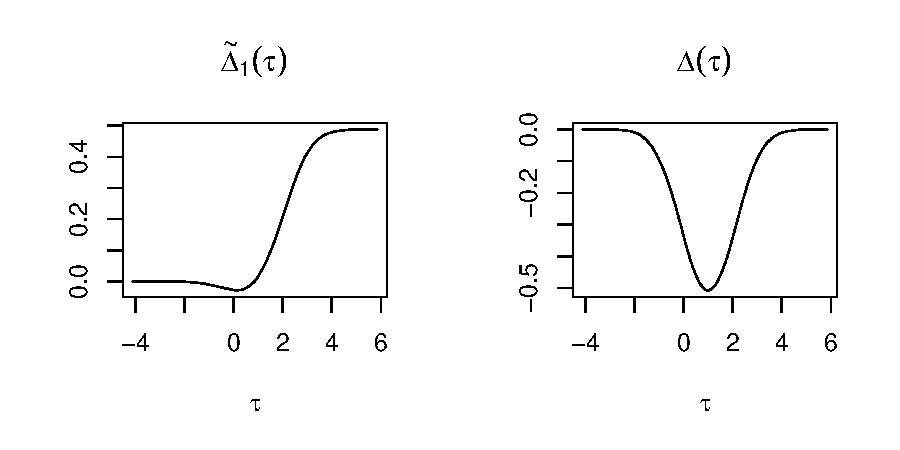
\includegraphics[width=\textwidth]{Delta_sim}
  \end{figure}
\[
    \widetilde{\Delta}_1(\tau+\beta) - \widetilde{\Delta}_1(\tau) = \alpha_0 \Delta(\tau + \beta) - (1 - \alpha_1) \Delta(\tau)
\]
\end{frame}
%%%%%%%%%%%%%%%%%%%%%%%%%%%%%%%%%%%%%

\begin{frame}
  \frametitle{Conclusion}
  %\singlespacing
  %\small

  \begin{block}{Summary}
  \begin{itemize}
    \item Endogenous, mis-measured binary treatment.
    \item Important in applied work but no solution in the literature.
      \item Usual (1st moment) IV assumption fails to identify $\beta$
      \item Bounds for mis-classification probabilities and $\beta$.
      \item Higher moment / independence restrictions identify $\beta$
   \end{itemize}
  \end{block}

  \begin{block}{Extensions / Work in Progress}
    \begin{itemize}
      \item Efficient estimation w/ continuum of MCs
        \item Inference / Specification Testing
      \item LATE interpretation
      \item Empirical Examples
    \end{itemize}
  \end{block}
\end{frame}
%%%%%%%%%%%%%%%%%%%%%%%%%%%%%%%%%%%%%%%
\appendix

\begin{frame}[label=MAHAJAN_APPEND]
  \frametitle{Mahajan (2006, ECTA)}

  \vspace{-1em}

    \begin{columns}[c]
    \column{.45\textwidth} 
    \begin{exampleblock}{Regression Model}
      $y = \mathbb{E}[y|T^*] + \nu$\\
      {\small $\mathbb{E}[\nu|T^*]=0$ by construction}
    \end{exampleblock}
    \column{.45\textwidth}
    \begin{exampleblock}{Causal Model}
     $y = c + \beta T^* + \varepsilon$\\
     {\small$\mathbb{E}[\varepsilon|T^*]\neq 0$}
    \end{exampleblock}
    \end{columns}

    \vspace{1.5em}
  
  \begin{block}{Main Result (Correct) -- Exogenous Treatment}
   Relevant binary instrument $z$ ($p^*_k \neq p^*_\ell$) identifies $\alpha_0, \alpha_1$ and $\mathbb{E}[y|T^*]$ provided that $\mathbb{E}[\nu|T^*,T,z]=0$ and $\alpha_0 + \alpha_1 < 1$. 
  \end{block}

  \begin{alertblock}{Extension (Incorrect) -- Endogenous Treatment}
    $\mathbb{E}[\varepsilon|z]=0$, $p^*_k \neq p^*_\ell$, $\mathbb{E}[\varepsilon|T,T^*,z]=\mathbb{E}[\varepsilon|T^*] \implies$ $\beta$ identified.
  \end{alertblock}

\end{frame}

%%%%%%%%%%%%%%%%%%%%%%%%%%%%%%%%%%%%%%

\begin{frame}
  \frametitle{Mahajan (2006, ECTA)}
    \begin{columns}[c]
    \column{.45\textwidth} 
    \begin{exampleblock}{Regression Model}
      $y = \mathbb{E}[y|T^*] + \nu$\\
      {\small $\mathbb{E}[\nu|T^*]=0$ by construction}
    \end{exampleblock}
    \column{.45\textwidth}
    \begin{exampleblock}{Causal Model}
     $y = c + \beta T^* + \varepsilon$\\
     {\small$\mathbb{E}[\varepsilon|T^*]\neq 0$}
    \end{exampleblock}
    \end{columns}

    \vspace{0.7em}

    \begin{block}{Ingredients}
      
  \begin{enumerate}
    \item If $p^*_k \neq p^*_\ell$, $\mathbb{E}[\varepsilon|z]=0$ then, since $\beta_{IV} = \beta/(1-\alpha_0-\alpha_1)$, knowledge of $\alpha_0,\alpha_1$ is sufficient to recover $\beta$. \textcolor{blue}{(Correct)}
    \item If $p^*_k \neq p^*_\ell$, $\mathbb{E}[\nu|T^*,T,z]=0$, $\alpha_0, \alpha_1$ are identified. \textcolor{blue}{(Correct)}
    \item[] \alert{\framebox{How to satisfy both 1 and 2 while allowing $\mathbb{E}[\varepsilon|T^*]\neq 0$?}}
    \item[3.] Assume that $\mathbb{E}[\varepsilon|T^*,T,z]=\mathbb{E}[\varepsilon|T^*]$ \\ {\small (i.e.\ $m_{0k}^* = m_{0\ell}^*$ and $m_{1k}^*=m_{1\ell}^*$)}
  \end{enumerate}
    \end{block}
\end{frame}
%%%%%%%%%%%%%%%%%%%%%%%%%%%%%%%%%%%%%%
\begin{frame}
  \frametitle{Flaw in the Argument}
  \begin{block}{Proposition}
    If $\mathbb{E}[\varepsilon|T^*]\neq 0$ then  $\mathbb{E}[\varepsilon|T^*,T,z]=\mathbb{E}[\varepsilon|T^*]$ combined with $\mathbb{E}[\varepsilon|z]=0$ implies $p^*_k = p^*_\ell$, i.e.\ $z$ is irrelevant for $T^*$.
  \end{block}
  \begin{block}{Proof}
    $\mathbb{E}[\varepsilon|z]=0$ implies
  \begin{align*}
    (1-p_1^*) \textcolor{red}{m^*_{0k}} + p^*_1 \textcolor{blue}{m^*_{1k}}&=c\\
    (1-p_2^*) \textcolor{red}{m^*_{0\ell}} + p^*_2 \textcolor{blue}{m^*_{1\ell}}&=c
  \end{align*}
  while Mahajan's assumption implies $m_{0k}^* = m_{0\ell}^*$ and $m_{1k}^*=m_{1\ell}^*$.
  Therefore either $m_{0k}^*=m_{0\ell}^* = m_{1k}^* =m_{1\ell}^*=c$, which is ruled out by $E[\varepsilon|T^*]=0$, or $p^*_k = p^*_\ell$.
  \end{block}
    \hyperlink{MAHAJAN_BODY}{\beamergotobutton{Back}}
\end{frame}
%%%%%%%%%%%%%%%%%%%%%%%%%%%%%%%%%%%%%%%
\end{document}
